% Options for packages loaded elsewhere
\PassOptionsToPackage{unicode}{hyperref}
\PassOptionsToPackage{hyphens}{url}
\PassOptionsToPackage{dvipsnames,svgnames,x11names}{xcolor}
%
\documentclass[
  letterpaper,
  DIV=11,
  numbers=noendperiod]{scrartcl}

\usepackage{amsmath,amssymb}
\usepackage{iftex}
\ifPDFTeX
  \usepackage[T1]{fontenc}
  \usepackage[utf8]{inputenc}
  \usepackage{textcomp} % provide euro and other symbols
\else % if luatex or xetex
  \usepackage{unicode-math}
  \defaultfontfeatures{Scale=MatchLowercase}
  \defaultfontfeatures[\rmfamily]{Ligatures=TeX,Scale=1}
\fi
\usepackage{lmodern}
\ifPDFTeX\else  
    % xetex/luatex font selection
\fi
% Use upquote if available, for straight quotes in verbatim environments
\IfFileExists{upquote.sty}{\usepackage{upquote}}{}
\IfFileExists{microtype.sty}{% use microtype if available
  \usepackage[]{microtype}
  \UseMicrotypeSet[protrusion]{basicmath} % disable protrusion for tt fonts
}{}
\makeatletter
\@ifundefined{KOMAClassName}{% if non-KOMA class
  \IfFileExists{parskip.sty}{%
    \usepackage{parskip}
  }{% else
    \setlength{\parindent}{0pt}
    \setlength{\parskip}{6pt plus 2pt minus 1pt}}
}{% if KOMA class
  \KOMAoptions{parskip=half}}
\makeatother
\usepackage{xcolor}
\setlength{\emergencystretch}{3em} % prevent overfull lines
\setcounter{secnumdepth}{-\maxdimen} % remove section numbering
% Make \paragraph and \subparagraph free-standing
\makeatletter
\ifx\paragraph\undefined\else
  \let\oldparagraph\paragraph
  \renewcommand{\paragraph}{
    \@ifstar
      \xxxParagraphStar
      \xxxParagraphNoStar
  }
  \newcommand{\xxxParagraphStar}[1]{\oldparagraph*{#1}\mbox{}}
  \newcommand{\xxxParagraphNoStar}[1]{\oldparagraph{#1}\mbox{}}
\fi
\ifx\subparagraph\undefined\else
  \let\oldsubparagraph\subparagraph
  \renewcommand{\subparagraph}{
    \@ifstar
      \xxxSubParagraphStar
      \xxxSubParagraphNoStar
  }
  \newcommand{\xxxSubParagraphStar}[1]{\oldsubparagraph*{#1}\mbox{}}
  \newcommand{\xxxSubParagraphNoStar}[1]{\oldsubparagraph{#1}\mbox{}}
\fi
\makeatother


\providecommand{\tightlist}{%
  \setlength{\itemsep}{0pt}\setlength{\parskip}{0pt}}\usepackage{longtable,booktabs,array}
\usepackage{calc} % for calculating minipage widths
% Correct order of tables after \paragraph or \subparagraph
\usepackage{etoolbox}
\makeatletter
\patchcmd\longtable{\par}{\if@noskipsec\mbox{}\fi\par}{}{}
\makeatother
% Allow footnotes in longtable head/foot
\IfFileExists{footnotehyper.sty}{\usepackage{footnotehyper}}{\usepackage{footnote}}
\makesavenoteenv{longtable}
\usepackage{graphicx}
\makeatletter
\newsavebox\pandoc@box
\newcommand*\pandocbounded[1]{% scales image to fit in text height/width
  \sbox\pandoc@box{#1}%
  \Gscale@div\@tempa{\textheight}{\dimexpr\ht\pandoc@box+\dp\pandoc@box\relax}%
  \Gscale@div\@tempb{\linewidth}{\wd\pandoc@box}%
  \ifdim\@tempb\p@<\@tempa\p@\let\@tempa\@tempb\fi% select the smaller of both
  \ifdim\@tempa\p@<\p@\scalebox{\@tempa}{\usebox\pandoc@box}%
  \else\usebox{\pandoc@box}%
  \fi%
}
% Set default figure placement to htbp
\def\fps@figure{htbp}
\makeatother
% definitions for citeproc citations
\NewDocumentCommand\citeproctext{}{}
\NewDocumentCommand\citeproc{mm}{%
  \begingroup\def\citeproctext{#2}\cite{#1}\endgroup}
\makeatletter
 % allow citations to break across lines
 \let\@cite@ofmt\@firstofone
 % avoid brackets around text for \cite:
 \def\@biblabel#1{}
 \def\@cite#1#2{{#1\if@tempswa , #2\fi}}
\makeatother
\newlength{\cslhangindent}
\setlength{\cslhangindent}{1.5em}
\newlength{\csllabelwidth}
\setlength{\csllabelwidth}{3em}
\newenvironment{CSLReferences}[2] % #1 hanging-indent, #2 entry-spacing
 {\begin{list}{}{%
  \setlength{\itemindent}{0pt}
  \setlength{\leftmargin}{0pt}
  \setlength{\parsep}{0pt}
  % turn on hanging indent if param 1 is 1
  \ifodd #1
   \setlength{\leftmargin}{\cslhangindent}
   \setlength{\itemindent}{-1\cslhangindent}
  \fi
  % set entry spacing
  \setlength{\itemsep}{#2\baselineskip}}}
 {\end{list}}
\usepackage{calc}
\newcommand{\CSLBlock}[1]{\hfill\break\parbox[t]{\linewidth}{\strut\ignorespaces#1\strut}}
\newcommand{\CSLLeftMargin}[1]{\parbox[t]{\csllabelwidth}{\strut#1\strut}}
\newcommand{\CSLRightInline}[1]{\parbox[t]{\linewidth - \csllabelwidth}{\strut#1\strut}}
\newcommand{\CSLIndent}[1]{\hspace{\cslhangindent}#1}

% TODO: Add custom LaTeX header directives here
\usepackage{booktabs}
\usepackage{caption}
\usepackage{longtable}
\usepackage{colortbl}
\usepackage{array}
\usepackage{anyfontsize}
\usepackage{multirow}
\usepackage{lineno}\linenumbers
\KOMAoption{captions}{tableheading}
\makeatletter
\@ifpackageloaded{caption}{}{\usepackage{caption}}
\AtBeginDocument{%
\ifdefined\contentsname
  \renewcommand*\contentsname{Table of contents}
\else
  \newcommand\contentsname{Table of contents}
\fi
\ifdefined\listfigurename
  \renewcommand*\listfigurename{List of Figures}
\else
  \newcommand\listfigurename{List of Figures}
\fi
\ifdefined\listtablename
  \renewcommand*\listtablename{List of Tables}
\else
  \newcommand\listtablename{List of Tables}
\fi
\ifdefined\figurename
  \renewcommand*\figurename{Figure}
\else
  \newcommand\figurename{Figure}
\fi
\ifdefined\tablename
  \renewcommand*\tablename{Table}
\else
  \newcommand\tablename{Table}
\fi
}
\@ifpackageloaded{float}{}{\usepackage{float}}
\floatstyle{ruled}
\@ifundefined{c@chapter}{\newfloat{codelisting}{h}{lop}}{\newfloat{codelisting}{h}{lop}[chapter]}
\floatname{codelisting}{Listing}
\newcommand*\listoflistings{\listof{codelisting}{List of Listings}}
\makeatother
\makeatletter
\makeatother
\makeatletter
\@ifpackageloaded{caption}{}{\usepackage{caption}}
\@ifpackageloaded{subcaption}{}{\usepackage{subcaption}}
\makeatother

\usepackage{bookmark}

\IfFileExists{xurl.sty}{\usepackage{xurl}}{} % add URL line breaks if available
\urlstyle{same} % disable monospaced font for URLs
\hypersetup{
  pdftitle={Projected warming will exceed the long-term thermal limits of rice cultivation},
  pdfauthor={Nicolas Gauthier; Ornob Alam; Michael D. Purugganan; Jade d'Alpoim-Guedes},
  colorlinks=true,
  linkcolor={blue},
  filecolor={Maroon},
  citecolor={Blue},
  urlcolor={Blue},
  pdfcreator={LaTeX via pandoc}}


\title{Projected warming will exceed the long-term thermal limits of
rice cultivation}
\author{Nicolas Gauthier \and Ornob Alam \and Michael D.
Purugganan \and Jade d'Alpoim-Guedes}
\date{}

\begin{document}
\maketitle
\begin{abstract}
Rice is a staple food for a significant portion of the global
population, particularly in Asia, where over one billion people rely on
it for daily subsistence. Understanding rice's historical thermal limits
is imperative for predicting how it will respond to future shifts in
global climate. Here, we integrate diverse records of contemporary rice
cultivation extent, archaeological data spanning rice's long-term
history since its earliest cultivation, and temperature projections for
the past, present, and future to assess how warm temperatures have
influenced and may continue to influence rice's geographical
distribution, productivity, and the adaptive strategies employed by
human societies to sustain this important crop. Our findings indicate a
consistent pattern over the past 10,000 years: domesticated Asian rice
varieties have seldom thrived in regions where the mean annual
temperature exceeds 28°C or warm-season maximum temperature exceeds
33°C. By the end of this century, climate projections estimate that the
land area exceeding this thermal threshold in Asia's major
rice-producing nations could expand by ten to thirty times. Our findings
have significant implications for global food security, as regions
heavily reliant on rice cultivation may encounter unprecedented
challenges in staple crop production under projected warming.
\end{abstract}


\newpage{}

\section{Introduction}\label{introduction}

Members of the grass family (\emph{Poaceae}), which include staples like
rice, maize, wheat, and barley, provide a majority of the global human
caloric intake. However, these crops face a looming threat: the rate of
anticipated climate change eclipses that of historical niche adaptations
in grasses. By 2070, temperatures are projected to rise at a rate 5,000
times faster than what most varieties of \emph{Poaceae} have experienced
throughout their evolution (\emph{1}). Historically, \emph{Poaceae}
experienced temperature shifts ranging from 1-8°C per million years, yet
future projections anticipate changes as swift as 0.02°C annually
(\emph{1}). Among these vital crops, domesticated Asian rice
(\emph{Oryza sativa}) serves as a primary food source for over half the
global population. More than 90\% of the world's rice is grown in Asia,
and one fifth of the world's population---more than 1 billion
people---depend on rice cultivation for their livelihood.

\emph{Oryza sativa} has a deep history of cultivation and domestication
beginning at least 7,000 years ago. Over the course of its domestication
and subsequent spread, Asian rice has made several adaptations to
changes in climate and has expanded well beyond its original range of
cultivation. Yet despite this expansion, rice exhibits a high degree of
niche conservatism compared to its wild progenitor (\emph{2}). Although
human selection---and, in recent decades, scientific breeding---can
accelerate the development of new traits far more rapidly than the
thousands of years wild plant species often require to adapt to new
climatic conditions, these advances have not successfully expanded
rice's thermal tolerance. Notably, as global temperatures rise, rice
farming has shifted from warmer areas to cooler ones rather than
adapting to increased heat (\emph{3}). Apparent increases in rice's
harvested area over recent decades largely reflect advances in farming
technology rather than an expansion of its climatic tolerance. For
example, rice cultivation in the People's Republic of China has
gradually extended northward from Central China into cooler regions, a
shift that, combined with intensified irrigation in the country's
hottest zones, has modestly increased rice yields and masked the adverse
effects of rising temperatures (\emph{3}, \emph{4}).

While some areas may benefit from warming temperatures (\emph{5}), this
trend is not universal. In many regions, smallholder farmers rely on
rice cultivation as their main source of income. Indeed, mismatches
between rice-harvested areas and overall environmental suitability
suggest that subsistence farming in low-income regions has already
stretched rice cultivation to its climatic boundaries (\emph{6}). To put
this into perspective, projections indicate that 15-40\% of India's
current rainfed rice cultivation zones will experience a reduction in
climatic suitability by 2050 (\emph{7}). Since 1974, 88\% of
rice-harvested areas show significant shifts in yield due to climatic
factors, with climate change reducing consumable food calories from rice
by 0.4\% compared to historical climate conditions (\emph{8}).

However, these findings are constrained by the current distributions of
rice cultivation and prevailing temperature. Few regions of the world
today experience the elevated temperatures projected in many future
climate-change scenarios. This makes it challenging to distinguish
between inherent thermal limits for rice growth and the practical
geographic constraints set by recent temperature distributions
(\emph{9}, \emph{10}). Global temperatures have already exceeded known
temperatures over the past 2,000 years and we are living in the warmest
centuries of at least the past 100,000 years (\emph{11}). Contemporary
studies of the thermal niche of rice have provided crucial insights into
specific regions and production systems, but those with a global scope
have often been reliant on limited datasets that may not capture the
full diversity of rice distributions. Challenges include the potential
underrepresentation of temperate rice varieties in China, uneven
sampling of rainfed or upland varieties, and the geographic scope of the
studies, which do not always encompass broad thermal ranges (\emph{4},
\emph{7}, \emph{9}). Archaeological studies have been instrumental in
documenting the timing and geographic trajectory of rice's domestication
and spread across Asia (\emph{12}--\emph{16}). Recent integration of
archaeological rice records with spatial paleoclimate reconstructions
has revealed that climate change played a major role in the early
diversification and spread of rice (\emph{17}, \emph{18}), but the
implications for rice's future adaptability have yet to be fully
explored.

Here, we integrate multiple lines of evidence from the extensive history
of rice cultivation to characterize the thermal range of rice and gauge
its potential adaptability to impending climate changes. By integrating
diverse records of the current extent of rice cultivation with
archaeological data on the distribution of rice since its earliest
cultivation and domestication, we aim to establish \emph{O. sativa's}
thermal limits---the temperature conditions under which rice has been
consistently cultivated throughout its domestication history. We
estimate long-term thermal limits associated with rice cultivation by
comparing contemporary estimates of rice extent with well-dated
archaeological rice occurrences, and complement this with genetic
analyses of adaptation potential in rice subspecies. We focus
specifically on Asian rice (\emph{O. sativa}) rather than African rice
(\emph{O. glaberrima}), as Asian rice comprises the vast majority of
global production and consumption and has the extensive archaeological
record necessary for long-term analysis. We use these results to assess
the impact of projected climate changes by the end of this century.
Together, our analyses confirm that imminent changes in climate
conditions may force large regions of today's primary rice producers to
confront mean annual, seasonal, and monthly peak temperatures
unprecedented in the history of rice cultivation and domestication.

\section{Results}\label{results}

We assess thermal limits on rice growth by comparing contemporary rice
extents estimated from satellite imagery, agricultural censuses, and
herbarium collections to indicators of annual and seasonal temperature
(Figure~\ref{fig-overview}). Our analysis combines present-day rice
extent data from diverse sources: satellite-based assessments of paddy
rice extent in Asia (\emph{19}), hybrid satellite/census evaluations of
global paddy rice cropping areas around the year 2000 (\emph{20}), and
global point occurrences derived from herbarium records and germplasm
accessions (\emph{22}). These datasets span a range of spatial scales,
time periods, production systems (e.g.~irrigated vs.~rainfed), and data
collection methods with complementary biases, allowing us to test the
robustness of these thermal limits across methodologically independent
data sources. We supplement this empirical work with reviews of rice's
response to warm temperatures from prior field and lab-based agronomic
studies.

\phantomsection\label{cell-fig-overview}
\begin{figure}[H]

\centering{

\pandocbounded{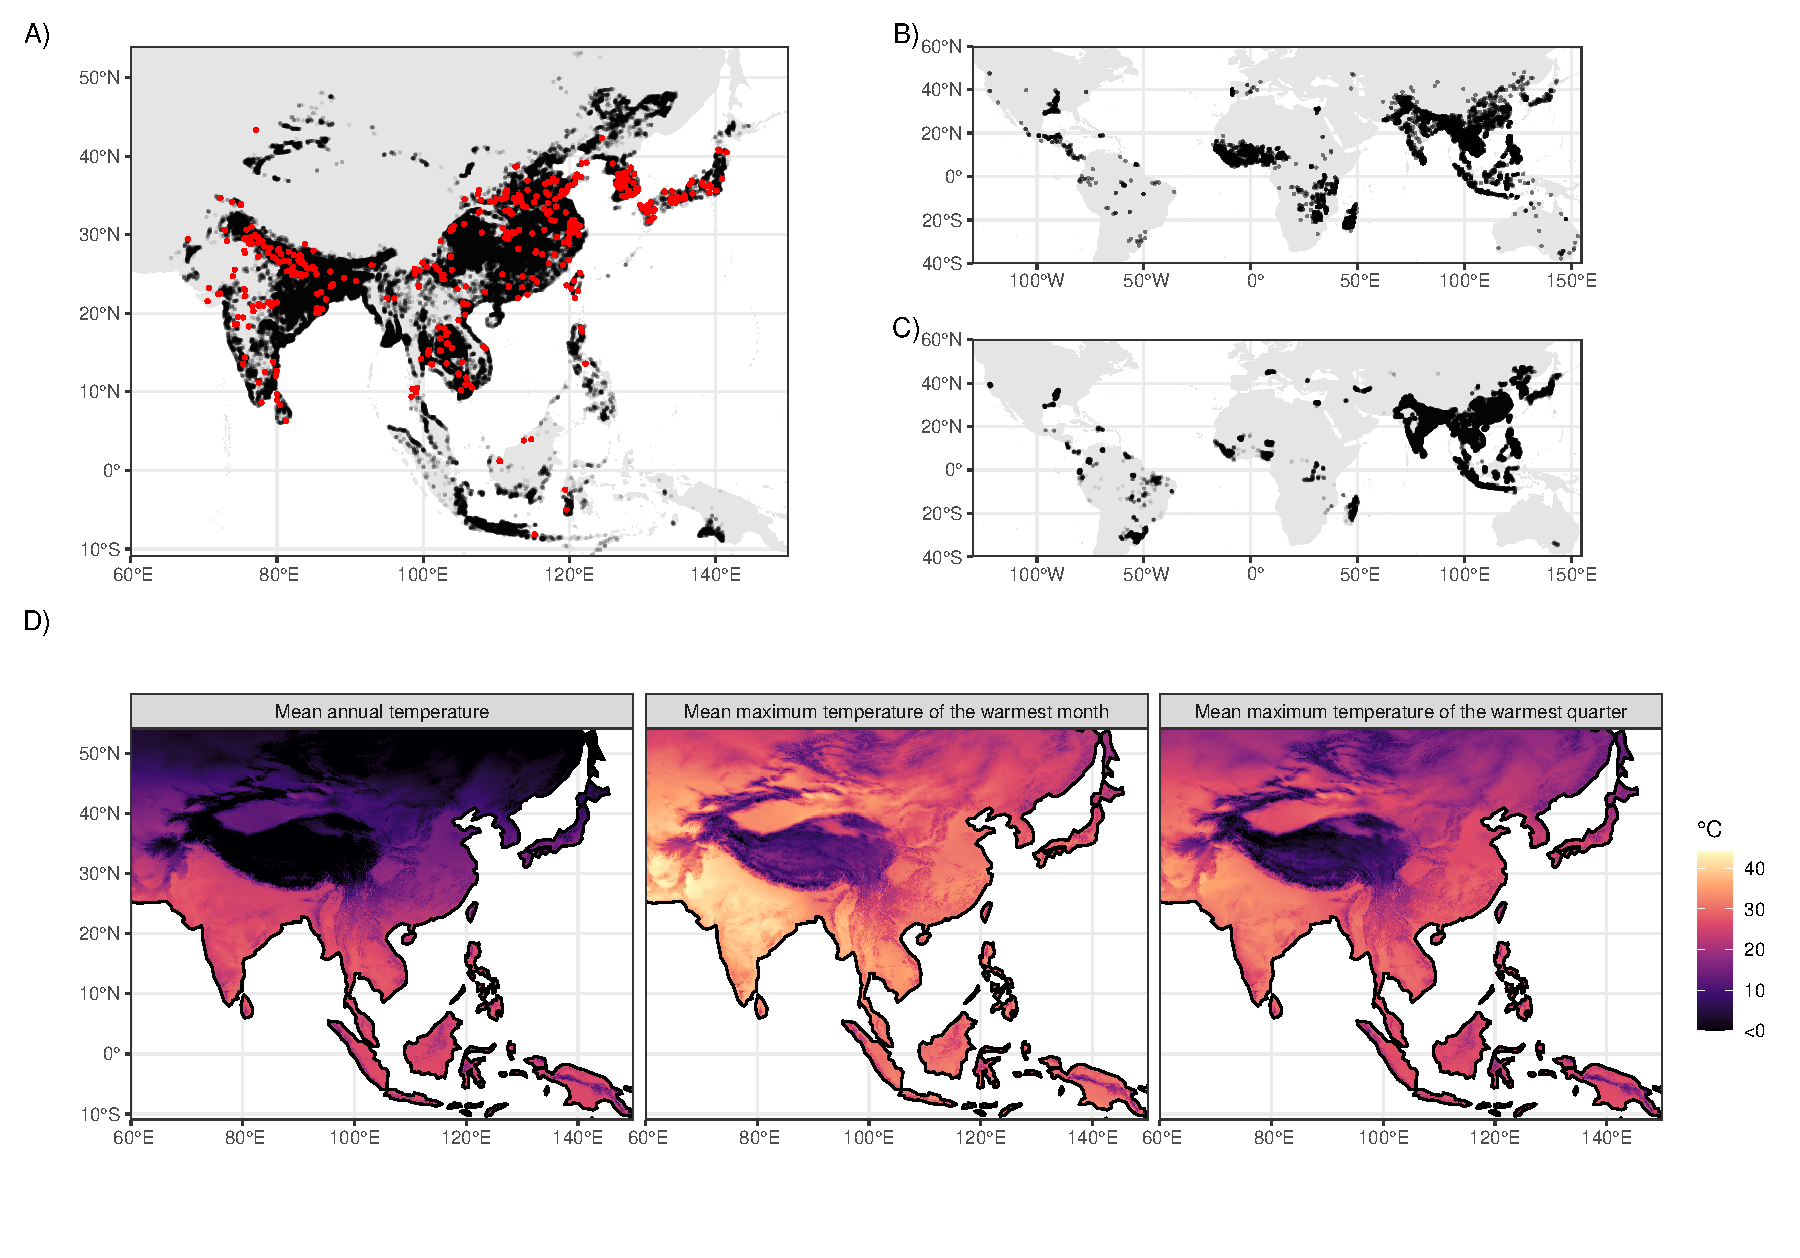
\includegraphics[keepaspectratio]{main_files/figure-pdf/fig-overview-1.pdf}}

}

\caption{\label{fig-overview}Observed rice extent data and thermal
predictors. A) Map of lowland rice extent in Asia from the International
Rice Research Institute based on estimates from MODIS satellite imagery
(\emph{19}) (black) overlain by archaeological sites with evidence for
rice cultivation (red). B) Point based rice occurrences from global
herbarium records and genetic accessions. C) Satellite-based estimates
of rice cropped area in the year 2000 from (\emph{20}). D) Maps of mean
annual temperature, mean maximum daily temperature of the warmest month,
and mean maximum daily temperature of the warmest quarter from CHELSA
V2.1 averages for 1981-2010 (\emph{23}--\emph{25}).}

\end{figure}%

We define the ``thermal limits'' of rice cultivation as the 95\% central
range of three temperature indicators at all sampled rice occurrence
locations in a given dataset---the temperature thresholds beyond which
the likelihood of rice cultivation significantly deceases due to a
combination of physiological, cultural, and economic factors. This
empirical approach emphasizes the long-term feasibility of crop
cultivation rather than short-term variations in yield or harvested
area. By focusing on these broader climatic measures, we can integrate a
wider array of data sources from the past and present to reveal the
upper temperature thresholds of rice cultivation over time.

Our approach offers a parsimonious tool for estimating future crop
suitability (\emph{26}, \emph{27}) that complements process-based crop
models. While such models can extrapolate yield responses to climate
change, they are sensitive to assumptions about meteorological inputs,
agronomic and physiological parameters, and cultural practices like
planting dates and varietal preferences over the long term
(\emph{28}--\emph{32}). Translating these localized projections to
global scales introduces additional challenges, as does calibrating and
validating their outputs using limited and inconsistent yield data from
the recent or more distant past. Ultimately, a better understanding of
baseline thermal limits and their uncertainty through time and space can
contribute to the development of future process-based models, many of
which incorporate temperature thresholds for pivotal crop development
phases.

We focus primarily on temperature rather than precipitation or soil
moisture, as water availability can be more readily controlled through
human interventions such as irrigation and paddy field construction.
These adaptations have allowed rice cultivation to expand beyond its
original aquatic and semi-aquatic environments. In contrast, adapting to
new thermal conditions is more challenging and often requires changes in
planting dates or crop varieties, which have their own limitations,
particularly in higher latitudes where daylight variations restrict
growing seasons.

\subsection{Contemporary rice extents are constrained by high
temperatures}\label{contemporary-rice-extents-are-constrained-by-high-temperatures}

Contemporary rice extents fall within a relatively restricted thermal
range. We use mean annual temperature (MAT), mean maximum daily
temperature of the warmest quarter (TWARM), and mean maximum daily
temperature of the warmest month (TMAX) to estimate upper boundary
temperatures for contemporary rice occurrences. The vast majority of
contemporary rice is grown in regions with MAT below 28.2℃, TWARM of
32.7℃, and TMAX of 40.4℃ (Figure~\ref{fig-kde-modern}). Although we
primarily report results from the satellite-based estimates of lowland
rice extent over Asia produced by the International Rice Research
Institute (\emph{19}) due to its favorable balance of spatial resolution
and extent, results from other rice extent datasets with variable
spatial extent, resolution, and time span are consistent with these
findings (Supplementary Table~\ref{tbl-quantiles}). There is much more
variability across data sources in lower temperature
thresholds---reflecting the greater adaptability of rice to colder
temperatures through breeding, management, and growing season---than
upper temperature thresholds.

\phantomsection\label{cell-fig-kde-modern}
\begin{figure}[H]

\centering{

\pandocbounded{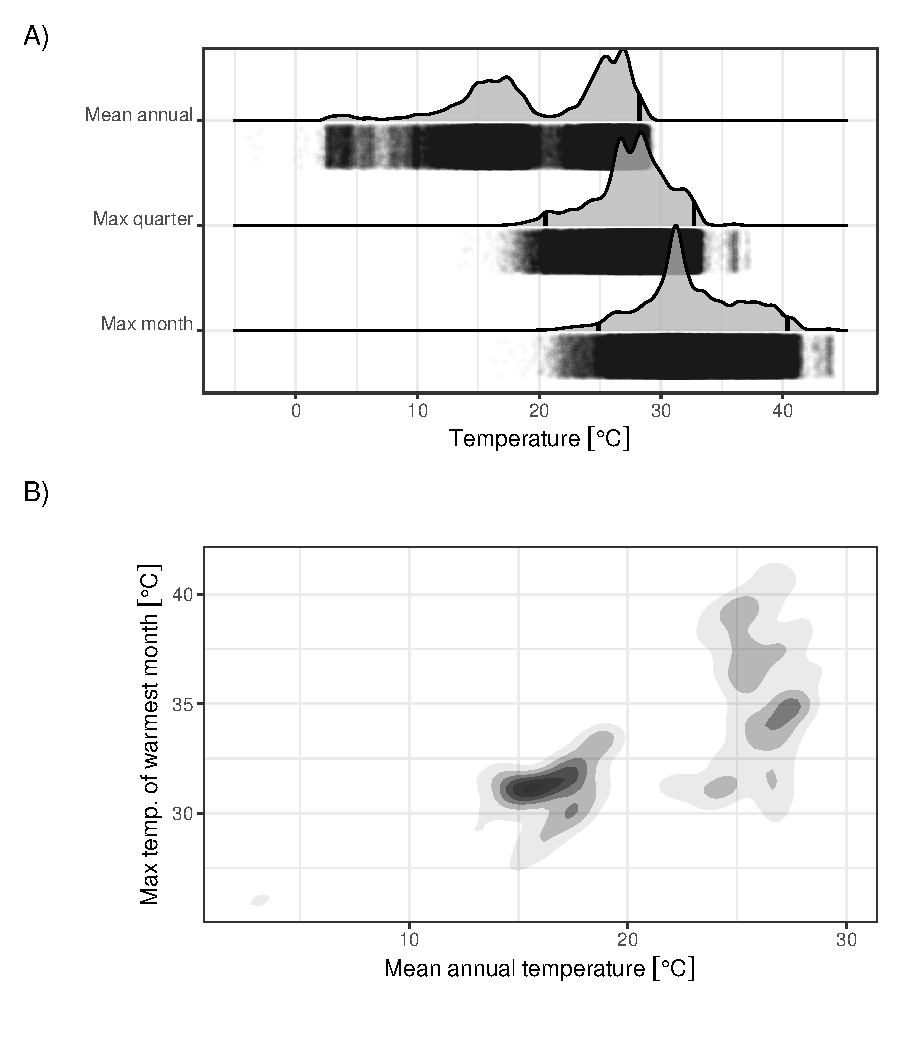
\includegraphics[keepaspectratio]{main_files/figure-pdf/fig-kde-modern-1.pdf}}

}

\caption{\label{fig-kde-modern}Kernel density estimates of temperature
distributions over rice growing landscapes in Asia. A) One-dimensional
kernel density estimates of mean annual temperature and mean maximum
daily temperature of the warmest month in grid cells with lowland rice
crops, based on data from the International Rice Research Institute
(fig.~1). Vertical black lines indicate the 95\% central range of the
temperature values, and transparent black points indicate the raw
occurrence data used in the calculation of the kernel density estimates.
B) Two dimensional kernel density estimates for the same variables as in
A.}

\end{figure}%

These empirical thresholds are consistent with physiological parameters
inferred from field-scale agronomic studies and expert knowledge, which
estimate that the optimum temperature range for reproductive yield in
rice is 23℃-26℃, biomass and pollen viability declines when maximum
temperatures exceed 33℃, and crop viability reaches zero at
approximately 40℃ when photosynthesis begins to shut down in C3 plants
like rice (\emph{33}). In other words, rice today is rarely grown in
regions where the mean annual temperature exceeds its optimum
temperature for reproduction, warm-season maximum temperatures exceed
its optimum for pollen viability, and summer heat extremes will reliably
stop photosynthesis.

These broad climate indices, while not capturing all nuances of local
growing conditions, serve as useful heuristics for identifying regions
prone to thermal stress. This approach provides a complementary
perspective to typical empirical crop models, which often use fixed
monthly or seasonal predictors tied to the timing of the growing season.
These predictors depend on planting dates, which are themselves cultural
adaptations to past and present climate. As planting times and growing
seasons shift with climate change, statistical analyses based solely on
``growing season'' temperatures may become less reliable for long-term
historical comparison. Our approach provides a stable benchmark for
integrating archaeological and contemporary data across different time
periods and cultivation practices, helping identify where adaptations in
growing seasons, crop types, genetics, or irrigation practices may
become necessary.

\subsection{High-temperature constraints are consistent across 9,000
years of rice
cultivation}\label{high-temperature-constraints-are-consistent-across-9000-years-of-rice-cultivation}

Although upper temperature limits on rice growth estimated from
contemporary crop occurrences are consistent with previous agronomic
studies, it is not yet clear how well these thresholds will predict crop
responses to future temperature changes. For example, there are few
places today that experience mean annual temperatures beyond 28℃
(Supplementary Figure \ref{fig-current-limits}), and contemporary
correlations between mean annual temperatures and monthly or seasonal
extremes may not hold in a changing climate. The archaeological record
of rice cultivation in Asia, including direct dates of botanical remains
and contextual dating of concurrent archaeological sites, provides a
unique opportunity to assess the robustness of these temperature limits
over the long term. During the mid Holocene ca 8000-4000 calibrated
years BP (cal. BP), warm-season temperatures were generally warmer than
present, reflecting increased summertime insolation in the Northern
Hemisphere due to shifts in Earth's orbit and consequent feedbacks in
the global climate system (\emph{34}). Although not an exact analogue
for projected future warming caused by greenhouse gas emissions, this
period provides a baseline for rice's response to shifting climates
during the critical period of its domestication and dispersal.

\emph{O. sativa} has been domesticated a number of times in prehistory.
Archaeological data shows that wild forms of rice were distributed as
far north as northern China in the early Holocene (ca 9000 cal. BP) and
gathered by foraging populations (\emph{35}). Tropical varieties of
\emph{O. sativa japonica} were first cultivated in the middle and lower
Yangtze and Yellow River valleys in China by at least 7000 cal. BP
(\emph{36}--\emph{38}) (Figure~\ref{fig-arch-kde} A), where they began
to exhibit traits of domestication (e.g.~the development of a
non-shattering rachis) by roughly 5000 cal. BP (\emph{12}, \emph{39}).
\emph{Oryza sativa indica} rices on the other hand were likely
domesticated in South Asia sometime around 4000 cal. BP (\emph{40},
\emph{41}), after which it spread throughout southeast Asia and China
(Figure~\ref{fig-arch-kde} A). There is substantially less
archaeobotanical data, however, that speaks to the cultivation and
subsequent domestication of this subspecies (\emph{41}). This period of
initial cultivation and domestication corresponds to the warmer
mid-Holocene thermal maximum.

Between roughly 5000-4000 BP, rice spread both north- and eastward in
China (\emph{42}, \emph{43}) and westward onto the Chengdu Plain
(\emph{44}) and highlands of Southwest China (\emph{45}, \emph{46})
(Figure~\ref{fig-arch-kde} A). Genetic and paleoclimate modeling have
suggested that regional cooling around 4200 BP played an important role
in this spread resulting in strong pressure for tropical \emph{O.
japonica} to develop temperate adaptations (\emph{18}). Estimated
divergence time for tropical and temperate \emph{O. japonica} is indeed
estimated at around 4100 BP (\emph{18}). Following the development of
temperate \emph{O. japonica} varieties, rice spread to both Korea
(\emph{47}, \emph{48}) and Japan (\emph{14}) (Figure~\ref{fig-arch-kde}
A). At the same time, it appears that the area that tropical varieties
of \emph{O. japonica} were able to occupy shifted southwards to southern
China (\emph{49}, \emph{50}) and southeast Asia (\emph{51}--\emph{53})
(Figure~\ref{fig-arch-kde} A), largely representing the dispersal of
existing tropical varieties rather than novel adaptations to new thermal
extremes. Indeed between 4000-3000 BP, rice farming spread into Thailand
(\emph{53}), Laos, Bhutan, and then via maritime routes to Taiwan, the
Philippines, Malaysia, and Indonesia (\emph{18})
(Figure~\ref{fig-arch-kde} A). A clear split in the distribution of rice
with regards to temperature is evident following 4000 BP and we see a
clear split into two populations: temperate varieties which occupy a
mean annual temperature niche between roughly 8-18℃ and tropical
varieties which occupy a niche between 22-27℃ (Figure~\ref{fig-arch-kde}
B).

\phantomsection\label{cell-fig-arch-kde}
\begin{figure}[H]

\centering{

\pandocbounded{\includegraphics[keepaspectratio]{main_files/figure-pdf/fig-arch-kde-1.pdf}}

}

\caption{\label{fig-arch-kde}Archaeological remains of rice and
corresponding temperature distributions throughout the Holocene. A.)
Archaeological records of rice distribution over time. See Materials and
Methods for archaeological data sources. Time units are thousands of
years before present (1950 CE). B.) Kernel density estimates of the
thermal distribution by millennium, with raw data points indicated in
black and contemporary rice thermal limits in red. Rice occurrence data
were derived from sources listed in the Materials and Methods.
Temperature data are derived from CHELSA-TraCE21k V1.0 (Karger et
al.~2023).}

\end{figure}%

These repeated instances of rice's diversification and shifting ranges
throughout its history primarily reflect genetic and cultural
adaptations to cooler temperatures and shorter growing seasons. In
contrast, movements into warmer regions generally involved range shifts
by varieties already suited to such conditions rather than novel
adaptations. Across these shifts, rice's upper temperature limits have
remained consistent. Out of 803 archaeological sites with rice remains,
none have experienced MAT of greater than 28.2℃ during the Holocene
(Figure~\ref{fig-arch-kde} B), in spite of warmer summer temperatures
overall. Only a handful of sites experienced a TMAX of greater than
40.4℃ (Figure~\ref{fig-arch-kde} C), primarily in arid regions of
northern India and Pakistan where archaeological dating is less certain
and long-distance trade rather than local cultivation is more plausible.
Regardless, the archaeological record of rice cultivation is consistent
with the thermal limits estimated from contemporary data, and these
results are robust to uncertainty in the dating of these archaeological
remains and spatial biases in archaeological site preservation and
recovery Supplementary Figure~\ref{fig-bootstrap}, as well as across
different climate reconstructions with varying degrees of mid-Holocene
warmth (Supplementary Figures \ref{fig-recon-timeseries} -
\ref{fig-kde-lgmr}).

\subsection{Currently cultivated rice areas are projected to exceed
these thermal limits over the next
century}\label{currently-cultivated-rice-areas-are-projected-to-exceed-these-thermal-limits-over-the-next-century}

Although rice has spread to warmer environments since its domestication,
the magnitude of this change over the past 9,000 years is small relative
to anticipated changes by the end of this century. Multiple
climate-model projections and future socioeconomic and emissions
scenarios show large shifts in annual and warm-season temperatures in
regions where rice is currently cultivated intensively, particularly in
South, Southeast and Island Southeast Asia
(Figure~\ref{fig-future-densities}). Mean annual temperature will exceed
28℃ for a substantial area of current occurrences in the years
2070-2100. Large parts of South, Southeast, and Island SE Asia will
experience temperature conditions for which there is no analogue in the
history of the cultivation and domestication of rice over at least the
past 9,000 years (Figure~\ref{fig-future-maps}, Supplementary Figure
\ref{fig-country-summaries}, Supplementary Tables 2-4). Although the
extent of these projected shifts vary among climate models and emissions
scenarios, the overall direction of this change is consistent
(Supplementary Figures 6-8).

\phantomsection\label{cell-fig-future-densities}
\begin{figure}[H]

\centering{

\pandocbounded{\includegraphics[keepaspectratio]{main_files/figure-pdf/fig-future-densities-1.pdf}}

}

\caption{\label{fig-future-densities}Predicted changes in biologically
relevant temperature indicators over currently cultivated rice areas in
Asia, relative to contemporary thermal thresholds (red dashed line).
Shared socioeconomic pathways (SSPs) are scenarios of projected
socioeconomic global changes used to derive greenhouse gas emission
scenarios. SSP1 is a best case scenario where global cooperation and
social and technological innovation are able to reduce greenhouse gas
emissions. SSP3 is a middle-range scenario characterized by high
population growth and global competition that hinders social and
technological innovation. SSP5 is a worst-case scenario characterized by
rapid economic growth and carbon emissions. All temperature estimates
are derived from CMIP6 climate model ensemble mean estimates for the
years 2071-2100, selected based on the ISIMIP3b protocol and downscaled
by the CHELSA-V2.1 algorithm.}

\end{figure}%

\phantomsection\label{cell-fig-future-maps}
\begin{figure}[H]

\centering{

\pandocbounded{\includegraphics[keepaspectratio]{main_files/figure-pdf/fig-future-maps-1.pdf}}

}

\caption{\label{fig-future-maps}Land areas projected to exceed each
temperature threshold by 2071-2100 from CMIP6 simulations, based on the
ISIMIP3b protocol and downscaled by CHELSA-V2.1. Color intensity
corresponds to the count of climate model ensemble members surpassing
the given threshold at each grid cell.}

\end{figure}%

While our spatial analyses reveal clear thermal boundaries in rice
distributions, understanding the potential genetic capacity for
adaptation provides added context to projected climate shifts. A genetic
offset analysis assessing the potential maladaptation of \emph{O.
sativa} subspecies to future climate scenarios, correlating contemporary
genetic variation with annual and seasonal temperature, indicates both
subspecies are at a significantly higher risk of maladaptation under
projected temperature regimes of the coming century
(Figure~\ref{fig-offsets}). Genetic offset analysis estimates how
climatically mismatched rice populations may become under future warming
by calculating the multidimensional distance between current allele
frequencies and those predicted to be adaptive under projected climate
conditions. The analysis produces unitless distance values where larger
numbers indicate populations whose current genetic makeup is more
divergent from what would be optimal for future climates, suggesting
higher vulnerability to climate-driven fitness declines. These distance
metrics synthesize information across multiple climate-responsive
genetic variants to forecast which populations face the greatest
adaptive challenges under temperature increases. When projecting to
future climates across Asia, optimal growing locations for rice
landraces (traditional crop varieties maintained by farmers and adapted
to local conditions) of both subspecies show a greater skew away from
the equator in the likeliest emissions scenarios (Supplemental Figure
\ref{fig-displacement}). For both \emph{japonica} and \emph{indica}, the
degree of maladaptation increases with worsening emissions scenarios,
but is generally greater than at any point experienced throughout the
Holocene.

\phantomsection\label{cell-fig-offsets}
\begin{figure}[H]

\centering{

\pandocbounded{\includegraphics[keepaspectratio]{main_files/figure-pdf/fig-offsets-1.pdf}}

}

\caption{\label{fig-offsets}Estimated genetic offsets of sampled rice
landraces for past and future scenarios relative to current baseline.
Each point represents a distinct population sampled for genetic
analysis. Higher genetic offsets indicate a greater degree of
maladaptation to the particular temperature regime. The ``past''
scenario reflects the highest modeled temperature at each location over
the past 12,000 years. The future scenarios are averaged across all
climate models in the ensemble.}

\end{figure}%

\section{Discussion}\label{discussion}

There is a clear upper limit of mean annual temperature over 28℃ and
warm-season maximum temperature over 33℃ for rice that has rarely been
crossed since its domestication. Forward looking climate projections
show that areas that currently house some of the highest densities of
rice cultivation on Earth will surpass this limit by the end of this
century (Figure~\ref{fig-future-maps}). Today, 675 million people live
in Southeast Asia and 1.9 billion people live in South Asia. By the end
of this century, it is estimated that at least this number of people
will live in the region that will surpass these thresholds. Today, mean
annual temperatures greater than 28℃ are distributed across only a very
small area of the planet which includes only a small portion of the gulf
desert and the Sahara (\emph{54}). Beyond the impact of this heat on
rice cultivation, this study raises serious concerns about the viability
of other temperature-sensitive crops in regions which will be impacted.
The predictions for these areas of the world are out of the historic
sample of distribution for rice and have no analogue in the present
climate.

While some regions, including parts of northern China and southern
Russia, may become climatically suitable for rice cultivation and could
even see yield gains as temperatures approach current optima (\emph{5},
e.g. \emph{55}, \emph{56}), such potential benefits will be highly
localized. Even if aggregate yields were to stabilize or increase in
some growing regions, they would not offset the immediate livelihood and
food security risks faced in regions projected to exceed current thermal
limits. Shifting rice production north to regions currently too cold to
grow rice will be insufficient to buffer these projected impacts. Beyond
the potential for unanticipated social and environmental impacts
(\emph{57}), this response would do little for the billions of people
who live in these hotter regions whose lives and livelihoods are
directly threatened. This response would also ignore that rice
cultivation requires extensive niche construction through the
construction of paddies and that abiotic factors such as sufficient
water for irrigation and soils which can accommodate paddy rice. Indeed,
many areas where rice is currently cultivated are already at the limit
of these secondary agronomic adaptations (\emph{6}). Ethnographic work
has shown that in Southeast Asia and China rice paddy soils have been
formed over thousands of years of continuous farming which has increased
their fertility (\emph{58}). Such long-term processes of niche
construction cannot be easily replaced.

Although we do not directly assess yields, regions projected to warm
beyond rice's historical thermal limits are likely to experience
sustained productivity declines without further adaptation, while some
cooler areas could benefit as temperatures approach present-day optima.
Both outcomes underscore the importance of adaptation strategies to
sustain production under shifting climatic conditions. Shifts in
planting dates to winter may provide solutions in some regions, but
higher temperatures are still a concern as rice is also sensitive to
warmer nighttime temperatures in the early growing period (\emph{59}).
While breeding for traits that improve resistance to heat stress, such
as early flowering (\emph{33}), offers some promise, large-scale
socio-cultural adaptations to new crop varieties---and, in some cases,
shifts in dietary preferences or staple composition (\emph{60})---imply
significant downstream impacts on regional cultures and economies that
can be difficult to anticipate and mitigate ahead of time. Additionally,
tropical varieties of \emph{O. japonica} will likely need to shift
northwards to higher latitudes, yet these varieties are highly sensitive
to day length, and the development of non-photosensitive temperate
\emph{O. japonica} may have taken thousands of years. More recent
efforts, however, such as the Green Revolution in Asia, achieved rapid
advances---including the development of non-photosensitive varieties
that enabled the expansion of rice cultivation into new latitudes
(\emph{61}).~A major breeding objective for the coming decades will thus
not only be to develop non-photosensitive varieties of tropical rice but
also matching cultivation strategies (e.g. \emph{62}) and associated
food system strategies and cultural norms.

The stored germplasm of landraces will thus serve as important genetic
resources to breed climate-adaptive loci into high-yielding commercial
rice varieties (\emph{63}--\emph{65}). Compared to modern cultivars,
landraces contain higher genetic diversity (\emph{66}, \emph{67}) and
adaptations to a wider range of climates (\emph{64}). This genetic
diversity can also be harnessed using traditional varietal mixtures and
diversified planting systems (\emph{68}), where growing complementary
crop varieties with different heat tolerances together can buffer
against temperature extremes. Maladaptation of rice landraces under
future climates may thus be amplified in modern cultivars and cropping
systems (\emph{69}). Although there is uncertainty in genomic offset
estimates due to model averaging across climate scenarios and
statistical uncertainty in genotype-environment associations, they
remain powerful predictors of maladaptation in projected climates
(\emph{70}). A warming climate also threatens wild relatives of rice and
the genetic resources they contain, which are currently largely limited
to South and Southeast Asia and cannot disperse as quickly without human
intervention (\emph{1}).

Our focus here on annual and seasonal temperature indicators allows for
the integration of a broader array of data and provides a more flexible
analysis that is less sensitive to uncertainty in cultivar type, growing
season, and local management practices. However, future work could
explore this variability further by developing new thermal indicators
more sensitive to the unique requirements of various cultivars, growing
seasons, and agro-ecological contexts. Temperature is not the only
climate variable that influences rice growth. Others like soil moisture
and solar radiation are also critical to rice growth in ways that,
likewise, depend on cultivar type, growing season, and management
practices. Extending this analysis to the global and regional climatic
drivers of local climate response of these multiple variables, such as
the influence of sea surface temperature variability and
atmosphere-ocean teleconnections, could provide further opportunities to
incorporate long-term climate reconstructions and projections of climate
impacts on rice viability. A more precise estimation of the long-range
correlations among key climate indicators in space and time, based on
long-term insights from the archaeological and paleoclimatological
record, would be particularly useful for developing holistic
recommendations for future agronomic and genetic adaptations.

Our interdisciplinary approach highlights a pressing reality: the vast
historical perspective of rice cultivation combined with past and
present climate data provide a sobering outlook for food security during
future climatic shifts. Staple food resources entrenched in centuries or
millennia of cultural and socio-economic development face unprecedented
challenges in the coming decades. The implications of these challenges
extend beyond agriculture and resonate through economic systems, trade
and migration flows, and deep-rooted cultural practices. The potential
displacement of rice cultivation zones suggests not merely a change in
global food patterns but a profound disruption of human societies rooted
in these agronomic traditions. Before us lies an urgent necessity for
international research, collaboration, and adaptive policy-making to
strengthen the resilience of this crop that sustains billions.

\section{Materials and Methods}\label{materials-and-methods}

\subsection{Climate Data}\label{climate-data}

We used high-resolution gridded climate data from version 2.1 of the
CHELSA product (\emph{71}). CHELSA incorporates bias-corrected outputs
from the ERA5 reanalysis (\emph{72}) with high-resolution terrain data
using mechanistic relationships between local climate and terrain.
Compared to other global gridded climate products, CHELSA offers
superior performance in mountainous regions, and its reliance on
high-quality reanalysis data instead of raw weather station data ensures
greater accuracy and internal consistency among climate variables.

For present-day observed climate, we used the CHELSA V2.1 product
spanning the period 1981-2010 at a 1km resolution. We further aggregated
the native 1km data to 5km and 10km grids to assess the sensitivity of
our results to the scale of the analysis, given the variable spatial
support of the contemporary rice extent data. In all cases we used
standard temperature indicators used in ecological niche modeling
studies (\emph{71}), derived from monthly climatologies of minimum and
maximum temperature, which collectively represent annual means, monthly
extremes, and seasonality. Future climate model ensembles were derived
from phase six of the Coupled Model Intercomparison Project (CMIP6)
(\emph{73}), using the subset of bias-corrected models and scenarios
used in phase 3b of the Inter-Sectoral Impact Model Intercomparison
Project (ISIMIP) (\emph{74}), bilinearly interpolated to the CHELSA V2.1
basemap using the delta change approach (\emph{25}).

Past climate data were primarily derived from the CHELSA-TraCE21k
product, a downscaled version of TraCE-21k simulation of the CCSM3
climate model spanning the last 21,000 years, at 100-year intervals
(\emph{76}). This product uses the older CHELSA V1.2 algorithm, along
with a trend-preserving bias correction and topographic correction for
shifting ice sheets across the deglacial period. While TraCE-21k has
known limitations (\emph{77}--\emph{80}), particularly in representing
mid-Holocene warmth, it was chosen for its unique combination of high
spatial resolution and seasonal temporal resolution necessary for
assessing rice cultivation conditions. To validate these findings, we
compared our results with other low-resolution mean annual temperature
reconstructions that show varying levels of mid-Holocene warmth
(\emph{81}, \emph{82}). Despite differences in overall temperature
trends, the key patterns in rice cultivation temperature distributions
remained consistent between reconstructions (fig.~S3).

\subsection{Contemporary Rice Distribution
Data}\label{contemporary-rice-distribution-data}

We collected rice occurrence data from a variety of sources combining
information from satellite imagery, administrative statistics, and
herbarium collections to assess the sensitivity of our results to
various modes of data collection, sampling, spatiotemporal scale, and
other potential sources of bias. These three distinct data types sample
different aspects of rice distribution with complementary biases.
Satellite estimates provide continuous spatial coverage but can
misclassify certain land cover types; census data offer detailed
regional production information but suffer from administrative reporting
issues and boundary effects; herbarium records provide precise,
ground-truthed identifications across diverse production systems but
show spatial bias in field accessibility and collection priorities. When
these data types with different sampling approaches converge on similar
thermal limits despite their distinct limitations, this suggests the
patterns are less likely to be methodological artifacts. The specific
datasets were:

\begin{itemize}
\item
  Satellite-based estimates of lowland rice extent in Asia from the
  International Rice Research Institute (\emph{19}). This dataset
  employs high-resolution (500m) presence-absence markers from MODIS
  observations (2000-2012) and offers relatively uniform sampling across
  both temperate and tropical regions. It provides a more objective
  approach than spatially biased occurrence records. However, its
  coverage is limited to East and Southeast Asia and it may poorly
  distinguish intercropped wheat and rice in Northeast China and natural
  wetlands and paddy rice cultivation in Indonesia. To minimize such
  sampling issues, we aggregated the 500m data into 5km grid cells,
  dropping occurrences with less than 20\% coverage to minimize false
  positives from low-pixel observations. Subsequent analyses of these
  data proved robust to the exact resolution and coverage threshold
  used.
\item
  Estimates of paddy rice harvested areas around the year 2000
  (\emph{20}). This dataset, integrates satellite-based estimates of
  cropland with sub-national statistics for rice harvested areas. It
  utilizes geospatial cropland maps to downscale harvest area and yield
  census data and offers global coverage at approximately 10km
  resolution. Countries that lack detailed administrative data at the
  subnational level, such as Laos and Kazakhstan, can exhibit overly
  smoothed areas. The use of harvested area as a metric can be
  misleading in regions with multiple annual harvests, leading to double
  or triple counting, but this is mitigated when converted to binary
  occurrence data.
\item
  Geolocated, point-based occurrence records for rice and its wild
  progenitor synthesized from previous studies (\emph{2}, \emph{18},
  \emph{21}, \emph{22}), originally sourced from GBIF, the Rice
  Haplotype Map project, and other datasets based on herbarium specimens
  or germplasm samples from international genebank databases. Given
  their direct identification, these occurrence records generally offer
  greater reliability than area-averaged crop occurrences derived from
  satellites and sub-national statistics. Nonetheless, they are
  susceptible to spatial sampling bias. For instance, regions like China
  are underrepresented in GBIF in terms of sampling effort compared to
  neighboring countries with similar geographical extent, and herbarium
  collections may more accurately sample upland rice varieties at the
  expense of larger paddy fields. After creating the full combined
  datasets, geolocations were checked for anomalous entries then thinned
  to a uniform grid to minimize irregular spatial sampling.
\end{itemize}

We extracted the contemporary CHELSA climate data at each set of
occurrence points for each data type to calculate temperature
distributions and quantiles. We explored various combinations of
grid/point resolution for the climate and occurrence datasets from
1-10km, but found this did not impact the upper temperature threshold
estimates.

\subsection{Archaeological Rice Distribution
Data}\label{archaeological-rice-distribution-data}

We used past rice occurrence data sourced from archaeological sites in
Asia, as synthesized in (\emph{83}) and (\emph{13}) and primarily
derived from version 2 (\emph{15}) and 3 (Dorian Fuller 2023, personal
communication) of the Rice Archaeological Database. We also included
observations from (\emph{14}) to increase data coverage in Japan. These
records are typically of botanical remains, believed to represent
\emph{O. sativa japonica} from these archaeological sites, with less
intensive sampling of \emph{indica} varieties from northern India.
However, based on their chronology, some occurrences might instead
reflect cultivation of wild-type \emph{O. rufipogon} or \emph{O.
nivara}. After data harmonization---which involved eliminating potential
outliers, correcting misclassifications, and removing duplicated site
data (see supplemental analysis code repository for the reproducible
workflow)---we were left with 1,595 dates from 803 archaeological sites.
These datasets comprise a mixture of direct radiocarbon dates on rice
remains, alongside dates for archaeological phases associated with rice
remains that were not directly dated. For these indirectly dated
samples, we used median dates and minimum/maximum date ranges for the
archaeological strata or contexts in which the rice remains were found.
We employed the Intcal20 calibration curve for recalibrating all
radiocarbon dates, barring a single site in the southern hemisphere
where we utilized SHcal20. We then extracted temperature variables from
the CHELSA-TraCE21k v1.0 dataset at each sampled location in time and
space. To account for chronological uncertainty, we generated 5,000
bootstrap replicates, sampling from the radiocarbon dates' posterior
density distribution and a uniform density for the dates based on
archaeological phases. Finally, we constructed unique kernel density
estimates of the temperature distributions at each rice occurrence point
for every bootstrap replicate and temperature variable.

\subsection{Genetic Offset Analysis}\label{genetic-offset-analysis}

To assess the adaptive capacity of rice varieties beyond simple
distributional limits, we performed a genetic offset analysis to
evaluate the potential maladaptation of \emph{Oryza sativa} subspecies
\emph{indica} and \emph{japonica} under projected climate change
scenarios. Genetic offset metrics provide a complementary perspective to
geographical threshold analyses by identifying where genetic adaptation
may or may not keep pace with changing thermal conditions. Landraces are
representative of the extant genetic diversity of crop species, and
frequently exhibit local adaptations from sustained cultivation in
specific geographic localities. We leveraged previously published
genomic datasets of geotagged rice landraces belonging to the subspecies
\emph{O. sativa ssp. Indica} (\emph{18}) and \emph{O. sativa ssp.
Japonica} (\emph{84}), containing genome-wide biallelic single
nucleotide polymorphisms (SNPs) filtered for quality and imputed for
missing genotypes. The workflow entailed a gene-environment association
analysis focusing on the first principal component of the three
temperature variables (MAT, TWARM, TMAX), which explained over 84\% of
the environmental variance across the locations of both rice subspecies.
Using the first principal component addresses multicollinearity among
the temperature variables while retaining most environmental variation.
The gene-environment association analysis was performed using the
\texttt{lfmm2} function from the R package LEA (v3.12.2)---on the two
subspecies separately---to identify variants associated with variation
in temperature (\emph{85}). To correct for population structure in the
GEA, we provided the number of ancestral populations, K, as the number
of latent factors in our latent factor mixed models (\emph{85}). We
selected the number of ancestral populations based on the number of
principal components of the genotype matrix that explain a large
proportion of the variance, the cross-entropy---a measure of model
fit---of different values of K, and information from prior studies
(\emph{18}, \emph{84}). Variants identified in the GEA were clumped
within 100 kilobases of each other, selecting the variant with the
lowest p-value as the candidate SNP from each linkage group. The genetic
offset, indicative of maladaptation to predicted climates (\emph{70}),
was calculated using these loci. These offset values indicate the
Euclidean distance between current genomic composition and the
composition theoretically required for adaptation to projected climate
conditions. We averaged model predictions across multiple climate models
(UKESM, MRI, IPSL, etc.) in the ensemble for each Shared Socioeconomic
Pathway (SSP).

We used the \texttt{genetic.offset} function of the R package LEA
(\emph{85}) to calculate genomic offset statistics for rice landraces of
\emph{O. sativa ssp. Indica} and \emph{O. sativa ssp. Japonica} while
considering the temperature-associated variants as putative adaptive
variants under the SSP1, SSP3, and SSP5 projected pathways that are used
to derive greenhouse gas emission scenarios. We also calculated genomic
offset statistics under the maximum estimated temperature at each
location in the past 12,000 years.

To make predictions about where the climate is likely to be optimal for
rice-growing in the future, we sampled 10,000 grids from across Asia and
calculated genomic offset scores for each individual in the environment
of each grid, for the three SSP scenarios. We interpret the grid with
the lowest offset score as a possible future optimal location for each
rice individual. As a measure of the extent of movement that would be
required for adaptation, we subtract the absolute value of the current
latitude of each rice individual from the absolute value of the centroid
latitude of the optimal grid; positive values of this absolute
latitudinal distance indicate movement away from the equator.

\section{References}\label{references}

\phantomsection\label{refs}
\begin{CSLReferences}{0}{1}
\bibitem[\citeproctext]{ref-cang2016}
\CSLLeftMargin{1. }%
\CSLRightInline{F. A. Cang, A. A. Wilson, J. J. Wiens,
\href{https://doi.org/10/gnjmsx}{Climate change is projected to outpace
rates of niche change in grasses}. \emph{Biology Letters} \textbf{12},
20160368 (2016).}

\bibitem[\citeproctext]{ref-yang2022}
\CSLLeftMargin{2. }%
\CSLRightInline{R. Yang, X. Gong, R. Cao, J. Feng,
\href{https://doi.org/10.1016/j.ecoinf.2022.101813}{Global niche shifts
of rice and its weak adaptability to climate change}. \emph{Ecological
Informatics} \textbf{71}, 101813 (2022).}

\bibitem[\citeproctext]{ref-sloat2020}
\CSLLeftMargin{3. }%
\CSLRightInline{L. L. Sloat, S. J. Davis, J. S. Gerber, F. C. Moore, D.
K. Ray, P. C. West, N. D. Mueller,
\href{https://doi.org/10.1038/s41467-020-15076-4}{Climate adaptation by
crop migration}. \emph{Nature Communications} \textbf{11}, 1243 (2020).}

\bibitem[\citeproctext]{ref-wang2019}
\CSLLeftMargin{4. }%
\CSLRightInline{H. Wang, R. J. Hijmans,
\href{https://doi.org/10.1088/2515-7620/ab0856}{Climate change and
geographic shifts in rice production in China}. \emph{Environmental
Research Communications} \textbf{1}, 011008 (2019).}

\bibitem[\citeproctext]{ref-gao2025cost}
\CSLLeftMargin{5. }%
\CSLRightInline{Y. Gao, J. Cui, X. Zhang, G. Hoogenboom, D. Wallach, Y.
Huang, S. Reis, T. Lin, B. Gu, Cost-effective adaptations increase rice
production while reducing pollution under climate change. \emph{Nature
Food} \textbf{6}, 260--272 (2025).}

\bibitem[\citeproctext]{ref-mahaut2022}
\CSLLeftMargin{6. }%
\CSLRightInline{L. Mahaut, S. Pironon, J.-Y. Barnagaud, F. Bretagnolle,
C. K. Khoury, Z. Mehrabi, R. Milla, C. Phillips, L. H. Rieseberg, C.
Violle, D. Renard, \href{https://doi.org/10.1098/rspb.2022.1542}{Matches
and mismatches between the global distribution of major food crops and
climate suitability}. \emph{Proceedings of the Royal Society B:
Biological Sciences} \textbf{289}, 20221542 (2022).}

\bibitem[\citeproctext]{ref-singh2017}
\CSLLeftMargin{7. }%
\CSLRightInline{K. Singh, C. J. McClean, P. Büker, S. E. Hartley, J. K.
Hill, \href{https://doi.org/10.1016/j.agsy.2017.05.009}{Mapping regional
risks from climate change for rainfed rice cultivation in India}.
\emph{Agricultural Systems} \textbf{156}, 76--84 (2017).}

\bibitem[\citeproctext]{ref-ray2019}
\CSLLeftMargin{8. }%
\CSLRightInline{D. K. Ray, P. C. West, M. Clark, J. S. Gerber, A. V.
Prishchepov, S. Chatterjee,
\href{https://doi.org/10.1371/journal.pone.0217148}{Climate change has
likely already affected global food production}. \emph{PLOS ONE}
\textbf{14}, e0217148 (2019).}

\bibitem[\citeproctext]{ref-welch2010}
\CSLLeftMargin{9. }%
\CSLRightInline{J. R. Welch, J. R. Vincent, M. Auffhammer, P. F. Moya,
A. Dobermann, D. Dawe,
\href{https://doi.org/10.1073/pnas.1001222107}{Rice yields in
tropical/subtropical asia exhibit large but opposing sensitivities to
minimum and maximum temperatures}. \emph{Proceedings of the National
Academy of Sciences} \textbf{107}, 14562--14567 (2010).}

\bibitem[\citeproctext]{ref-soberuxf3n2017}
\CSLLeftMargin{10. }%
\CSLRightInline{J. Soberón, B. Arroyo-Peña,
\href{https://doi.org/10.1371/journal.pone.0175138}{Are fundamental
niches larger than the realized? Testing a 50-year-old prediction by
Hutchinson}. \emph{PLOS ONE} \textbf{12}, e0175138 (2017).}

\bibitem[\citeproctext]{ref-masson-delmotte2021}
\CSLLeftMargin{11. }%
\CSLRightInline{V. Masson-Delmotte, P. Zhai, A. Pirani, S. L. Connors,
C. Péan, S. Berger, N. Caud, Y. Chen, L. Goldfarb, M. Gomis, others,
Climate change 2021: The physical science basis. \emph{Contribution of
working group I to the sixth assessment report of the intergovernmental
panel on climate change} \textbf{2} (2021).}

\bibitem[\citeproctext]{ref-fuller2009}
\CSLLeftMargin{12. }%
\CSLRightInline{D. Q. Fuller, L. Qin, Y. Zheng, Z. Zhao, X. Chen, L. A.
Hosoya, G.-P. Sun, \href{https://doi.org/10.1126/science.1166605}{The
Domestication Process and Domestication Rate in Rice: Spikelet Bases
from the Lower Yangtze}. \emph{Science} \textbf{323}, 1607--1610
(2009).}

\bibitem[\citeproctext]{ref-long2022}
\CSLLeftMargin{13. }%
\CSLRightInline{T. Long, H. Chen, C. Leipe, M. Wagner, P. E. Tarasov,
\href{https://doi.org/10.1016/j.quaint.2021.11.016}{Modelling the
chronology and dynamics of the spread of Asian rice from ca. 8000 BCE to
1000 CE}. \emph{Quaternary International} \textbf{623}, 101--109
(2022).}

\bibitem[\citeproctext]{ref-crema2022}
\CSLLeftMargin{14. }%
\CSLRightInline{E. R. Crema, C. J. Stevens, S. Shoda,
\href{https://doi.org/10.1126/sciadv.adc9171}{Bayesian analyses of
direct radiocarbon dates reveal geographic variations in the rate of
rice farming dispersal in prehistoric Japan}. \emph{Science Advances}
\textbf{8}, eadc9171 (2022).}

\bibitem[\citeproctext]{ref-silva2015}
\CSLLeftMargin{15. }%
\CSLRightInline{F. Silva, C. J. Stevens, A. Weisskopf, C. Castillo, L.
Qin, A. Bevan, D. Q. Fuller,
\href{https://doi.org/10.1371/journal.pone.0137024}{Modelling the
Geographical Origin of Rice Cultivation in Asia Using the Rice
Archaeological Database}. \emph{PLOS ONE} \textbf{10}, e0137024 (2015).}

\bibitem[\citeproctext]{ref-weber2010}
\CSLLeftMargin{16. }%
\CSLRightInline{S. Weber, H. Lehman, T. Barela, S. Hawks, D. Harriman,
\href{https://doi.org/10.1007/s12520-010-0030-3}{Rice or millets: early
farming strategies in prehistoric central Thailand}.
\emph{Archaeological and Anthropological Sciences} \textbf{2}, 79--88
(2010).}

\bibitem[\citeproctext]{ref-dalpoimguedes2018}
\CSLLeftMargin{17. }%
\CSLRightInline{J. d'Alpoim Guedes, R. K. Bocinsky,
\href{https://doi.org/10/gfkwf8}{Climate change stimulated agricultural
innovation and exchange across Asia}. \emph{Science Advances}
\textbf{4}, eaar4491 (2018).}

\bibitem[\citeproctext]{ref-gutaker2020}
\CSLLeftMargin{18. }%
\CSLRightInline{R. M. Gutaker, S. C. Groen, E. S. Bellis, J. Y. Choi, I.
S. Pires, R. K. Bocinsky, E. R. Slayton, O. Wilkins, C. C. Castillo, S.
Negrão, M. M. Oliveira, D. Q. Fuller, J. A. d'Alpoim. Guedes, J. R.
Lasky, M. D. Purugganan, \href{https://doi.org/10/ggx54g}{Genomic
history and ecology of the geographic spread of rice}. \emph{Nature
Plants} \textbf{6}, 492--502 (2020).}

\bibitem[\citeproctext]{ref-nelson2015}
\CSLLeftMargin{19. }%
\CSLRightInline{A. Nelson, M. K. Gumma, A map of lowland rice extent in
the major rice growing countries of {Asia} (2015).}

\bibitem[\citeproctext]{ref-monfreda2008}
\CSLLeftMargin{20. }%
\CSLRightInline{C. Monfreda, N. Ramankutty, J. A. Foley,
\href{https://doi.org/10.1029/2007GB002947}{Farming the planet: 2.
Geographic distribution of crop areas, yields, physiological types, and
net primary production in the year 2000}. \emph{Global Biogeochemical
Cycles} \textbf{22}, 2007GB002947 (2008).}

\bibitem[\citeproctext]{ref-civuxe1n2018}
\CSLLeftMargin{21. }%
\CSLRightInline{P. Civáň, T. A. Brown,
\href{https://doi.org/10.1186/s12862-018-1180-7}{Role of genetic
introgression during the evolution of cultivated rice (oryza sativa
l.)}. \emph{BMC Evolutionary Biology} \textbf{18}, 57 (2018).}

\bibitem[\citeproctext]{ref-ramirez-villegas2022}
\CSLLeftMargin{22. }%
\CSLRightInline{J. Ramirez-Villegas, C. K. Khoury, H. A. Achicanoy, M.
V. Diaz, A. C. Mendez, C. C. Sosa, Z. Kehel, L. Guarino, M. Abberton, J.
Aunario, B. A. Awar, J. C. Alarcon, A. Amri, N. L. Anglin, V. Azevedo,
K. Aziz, G. L. Capilit, O. Chavez, D. Chebotarov, D. E. Costich, D. G.
Debouck, D. Ellis, H. Falalou, A. Fiu, M. E. Ghanem, P. Giovannini, A.
J. Goungoulou, B. Gueye, A. I. E. Hobyb, R. Jamnadass, C. S. Jones, B.
Kpeki, J.-S. Lee, K. L. McNally, A. Muchugi, M.-N. Ndjiondjop, O.
Oyatomi, T. S. Payne, S. Ramachandran, G. Rossel, N. Roux, M. Ruas, C.
Sansaloni, J. Sardos, T. D. Setiyono, M. Tchamba, I. van den Houwe, J.
A. Velazquez, R. Venuprasad, P. Wenzl, M. Yazbek, C. Zavala,
\href{https://doi.org/10.1038/s41477-022-01144-8}{State of ex situ
conservation of landrace groups of 25 major crops}. \emph{Nature Plants}
\textbf{8}, 491--499 (2022).}

\bibitem[\citeproctext]{ref-karger2017}
\CSLLeftMargin{23. }%
\CSLRightInline{D. N. Karger, O. Conrad, J. Böhner, T. Kawohl, H. Kreft,
R. W. Soria-Auza, N. E. Zimmermann, H. P. Linder, M. Kessler,
\href{https://doi.org/10.1038/sdata.2017.122}{Climatologies at high
resolution for the earth{'}s land surface areas}. \emph{Scientific Data}
\textbf{4}, 170122 (2017).}

\bibitem[\citeproctext]{ref-Karger2018}
\CSLLeftMargin{24. }%
\CSLRightInline{D. N. Karger, O. Conrad, J. Böhner, T. Kawohl, H. Kreft,
R. W. Soria-Auza, N. E. Zimmermann, H. P. Linder, M. Kessler, Data from:
Climatologies at high resolution for the earth's land surface areas.
doi: \href{https://doi.org/10.5061/dryad.kd1d4}{10.5061/dryad.kd1d4}
(2018).}

\bibitem[\citeproctext]{ref-brun2022}
\CSLLeftMargin{25. }%
\CSLRightInline{P. Brun, N. E. Zimmermann, C. Hari, L. Pellissier, D. N.
Karger, {``Global climate-related predictors at kilometre resolution for
the past and future''} (2022);
\url{https://doi.org/10.5194/essd-2022-212}.}

\bibitem[\citeproctext]{ref-hatfield2011}
\CSLLeftMargin{26. }%
\CSLRightInline{J. L. Hatfield, K. J. Boote, B. A. Kimball, L. H. Ziska,
R. C. Izaurralde, D. Ort, A. M. Thomson, D. Wolfe,
\href{https://doi.org/10.2134/agronj2010.0303}{Climate Impacts on
Agriculture: Implications for Crop Production}. \emph{Agronomy Journal}
\textbf{103}, 351--370 (2011).}

\bibitem[\citeproctext]{ref-Gourdji2012}
\CSLLeftMargin{27. }%
\CSLRightInline{S. M. Gourdji, K. L. Mathews, M. Reynolds, D. B. Lobell,
S. M. Gourdji, An assessment of wheat yield sensitivity and breeding
gains in hot environments. (2012).}

\bibitem[\citeproctext]{ref-zhang2008}
\CSLLeftMargin{28. }%
\CSLRightInline{T. Zhang, J. Zhu, X. Yang,
\href{https://doi.org/10.1016/j.agrformet.2008.04.007}{Non-stationary
thermal time accumulation reduces the predictability of climate change
effects on agriculture}. \emph{Agricultural and Forest Meteorology}
\textbf{148}, 1412--1418 (2008).}

\bibitem[\citeproctext]{ref-vanoort2011}
\CSLLeftMargin{29. }%
\CSLRightInline{P. A. J. van Oort, T. Zhang, M. E. de Vries, A. B.
Heinemann, H. Meinke,
\href{https://doi.org/10.1016/j.agrformet.2011.06.012}{Correlation
between temperature and phenology prediction error in rice ({\emph{Oryza
sativa}} l.)}. \emph{Agricultural and Forest Meteorology} \textbf{151},
1545--1555 (2011).}

\bibitem[\citeproctext]{ref-li2015}
\CSLLeftMargin{30. }%
\CSLRightInline{T. Li, T. Hasegawa, X. Yin, Y. Zhu, K. Boote, M. Adam,
S. Bregaglio, S. Buis, R. Confalonieri, T. Fumoto, D. Gaydon, M.
Marcaida III, H. Nakagawa, P. Oriol, A. C. Ruane, F. Ruget, B.-. Singh,
U. Singh, L. Tang, F. Tao, P. Wilkens, H. Yoshida, Z. Zhang, B. Bouman,
\href{https://doi.org/10.1111/gcb.12758}{Uncertainties in predicting
rice yield by current crop models under a wide range of climatic
conditions}. \emph{Global Change Biology} \textbf{21}, 1328--1341
(2015).}

\bibitem[\citeproctext]{ref-koehler2013}
\CSLLeftMargin{31. }%
\CSLRightInline{A.-K. Koehler, A. J. Challinor, E. Hawkins, S. Asseng,
\href{https://doi.org/10.1088/1748-9326/8/3/034016}{Influences of
increasing temperature on Indian wheat: quantifying limits to
predictability}. \emph{Environmental Research Letters} \textbf{8},
034016 (2013).}

\bibitem[\citeproctext]{ref-heinicke2022}
\CSLLeftMargin{32. }%
\CSLRightInline{S. Heinicke, K. Frieler, J. Jägermeyr, M. Mengel,
\href{https://doi.org/10.1088/1748-9326/ac592e}{Global gridded crop
models underestimate yield responses to droughts and heatwaves}.
\emph{Environmental Research Letters} \textbf{17}, 044026 (2022).}

\bibitem[\citeproctext]{ref-ren2023}
\CSLLeftMargin{33. }%
\CSLRightInline{H. Ren, J. Bao, Z. Gao, D. Sun, S. Zheng, J. Bai,
\href{https://doi.org/10.3389/fpls.2023.1137923}{How rice adapts to high
temperatures}. \emph{Frontiers in Plant Science} \textbf{14} (2023).}

\bibitem[\citeproctext]{ref-berger1991}
\CSLLeftMargin{34. }%
\CSLRightInline{A. Berger, M. F. Loutre,
\href{https://doi.org/10.1016/0277-3791(91)90033-Q}{Insolation values
for the climate of the last 10 million years}. \emph{Quaternary Science
Reviews} \textbf{10}, 297--317 (1991).}

\bibitem[\citeproctext]{ref-fuller2011}
\CSLLeftMargin{35. }%
\CSLRightInline{D. Q. Fuller,
\href{https://doi.org/10.1007/s12284-011-9078-7}{Pathways to Asian
Civilizations: Tracing the Origins and Spread of Rice and Rice
Cultures}. \emph{Rice} \textbf{4}, 78--92 (2011).}

\bibitem[\citeproctext]{ref-huang2012}
\CSLLeftMargin{36. }%
\CSLRightInline{X. Huang, N. Kurata, X. Wei, Z.-X. Wang, A. Wang, Q.
Zhao, Y. Zhao, K. Liu, H. Lu, W. Li, Y. Guo, Y. Lu, C. Zhou, D. Fan, Q.
Weng, C. Zhu, T. Huang, L. Zhang, Y. Wang, L. Feng, H. Furuumi, T. Kubo,
T. Miyabayashi, X. Yuan, Q. Xu, G. Dong, Q. Zhan, C. Li, A. Fujiyama, A.
Toyoda, T. Lu, Q. Feng, Q. Qian, J. Li, B. Han,
\href{https://doi.org/10.1038/nature11532}{A map of rice genome
variation reveals the origin of cultivated rice}. \emph{Nature}
\textbf{490}, 497--501 (2012).}

\bibitem[\citeproctext]{ref-choi2017}
\CSLLeftMargin{37. }%
\CSLRightInline{J. Y. Choi, A. E. Platts, D. Q. Fuller, Y.-I. Hsing
(邢禹依), R. A. Wing, M. D. Purugganan,
\href{https://doi.org/10.1093/molbev/msx049}{The rice paradox: Multiple
origins but single domestication in asian rice}. \emph{Molecular Biology
and Evolution} \textbf{34}, 969--979 (2017).}

\bibitem[\citeproctext]{ref-choi2018}
\CSLLeftMargin{38. }%
\CSLRightInline{J. Y. Choi, M. D. Purugganan,
\href{https://doi.org/10.1534/g3.117.300334}{Multiple origin but single
domestication led to oryza sativa}. \emph{G3
Genes\textbar Genomes\textbar Genetics} \textbf{8}, 797--803 (2018).}

\bibitem[\citeproctext]{ref-Silva2015}
\CSLLeftMargin{39. }%
\CSLRightInline{F. Silva, C. J. Stevens, A. Weisskopf, C. Castillo, L.
Qin, A. Bevan, D. Q. Fuller,
\href{https://doi.org/10.1371/journal.pone.0137024}{Modelling the
geographical origin of rice cultivation in asia using the rice
archaeological database}. 1--21 (2015).}

\bibitem[\citeproctext]{ref-fuller2016}
\CSLLeftMargin{40. }%
\CSLRightInline{D. Q. Fuller, A. R. Weisskopf, C. Castillo,
\href{http://doi.\%20org/10.5334/ai.1915}{Pathways of Rice
Diversification across Asia}. \emph{Archaeology International}
\textbf{19}, 84--96 (2016).}

\bibitem[\citeproctext]{ref-bates2022}
\CSLLeftMargin{41. }%
\CSLRightInline{J. Bates,
\href{https://doi.org/10.3389/fevo.2022.924977}{The fits and starts of
indian rice domestication: How the movement of rice across northwest
india impacted domestication pathways and agricultural stories}.
\emph{Frontiers in Ecology and Evolution} \textbf{10} (2022).}

\bibitem[\citeproctext]{ref-lanehart2011}
\CSLLeftMargin{42. }%
\CSLRightInline{R. E. Lanehart, R. H. Tykot, A. P. Underhill, F. Luan,
H. Yu, H. Fang, C. Fengshu, G. Feinman, L. Nicholas,
\href{https://doi.org/10.1016/j.jas.2011.03.011}{Dietary adaptation
during the Longshan period in China: stable isotope analyses at
Liangchengzhen (southeastern Shandong)}. \emph{Journal of Archaeological
Science} \textbf{38}, 2171--2181 (2011).}

\bibitem[\citeproctext]{ref-dalpoimguedes2015}
\CSLLeftMargin{43. }%
\CSLRightInline{J. d'Alpoim Guedes, G. Jin, R. K. Bocinsky,
\href{https://doi.org/10/f7sgnj}{The Impact of Climate on the Spread of
Rice to North-Eastern China: A New Look at the Data from Shandong
Province}. \emph{PLOS ONE} \textbf{10}, e0130430 (2015).}

\bibitem[\citeproctext]{ref-dalpoimguedes2013}
\CSLLeftMargin{44. }%
\CSLRightInline{J. d'Alpoim Guedes, M. Jiang, K. He, X. Wu, Z. Jiang,
\href{https://doi.org/10.1017/S0003598X00049449}{Site of Baodun yields
earliest evidence for the spread of rice and foxtail millet agriculture
to south-west China}. \emph{Antiquity} \textbf{87}, 758--771 (2013).}

\bibitem[\citeproctext]{ref-dalpoimguedes2014}
\CSLLeftMargin{45. }%
\CSLRightInline{J. d'Alpoim Guedes, E. E. Butler,
\href{https://doi.org/10/f6qj7q}{Modeling constraints on the spread of
agriculture to Southwest China with thermal niche models}.
\emph{Quaternary International} \textbf{349}, 29--41 (2014).}

\bibitem[\citeproctext]{ref-dalmartello2018}
\CSLLeftMargin{46. }%
\CSLRightInline{R. Dal Martello, R. Min, C. Stevens, C. Higham, T.
Higham, L. Qin, D. Q. Fuller,
\href{https://doi.org/10.1016/j.jasrep.2018.06.005}{Early agriculture at
the crossroads of China and Southeast Asia: Archaeobotanical evidence
and radiocarbon dates from Baiyangcun, Yunnan}. \emph{Journal of
Archaeological Science: Reports} \textbf{20}, 711--721 (2018).}

\bibitem[\citeproctext]{ref-crawford2003}
\CSLLeftMargin{47. }%
\CSLRightInline{G. W. Crawford, G.-A. Lee,
\href{https://doi.org/10.1017/S0003598X00061378}{Agricultural origins in
the Korean Peninsula}. \emph{Antiquity} \textbf{77}, 87--95 (2003).}

\bibitem[\citeproctext]{ref-ahn2010}
\CSLLeftMargin{48. }%
\CSLRightInline{S.-M. Ahn,
\href{https://doi.org/10.1007/s12520-010-0029-9}{The emergence of rice
agriculture in Korea: archaeobotanical perspectives}.
\emph{Archaeological and Anthropological Sciences} \textbf{2}, 89--98
(2010).}

\bibitem[\citeproctext]{ref-yang2017}
\CSLLeftMargin{49. }%
\CSLRightInline{X. Yang, W. Wang, Y. Zhuang, Z. Li, Z. Ma, Y. Ma, Y.
Cui, J. Wei, D. Q. Fuller,
\href{https://doi.org/10.1177/0959683616678465}{New radiocarbon evidence
on early rice consumption and farming in South China}. \emph{The
Holocene} \textbf{27}, 1045--1051 (2017).}

\bibitem[\citeproctext]{ref-deng2022}
\CSLLeftMargin{50. }%
\CSLRightInline{Z. Deng, B. Huang, Q. Zhang, M. Zhang,
\href{https://doi.org/10.3389/feart.2022.858492}{First farmers in the
south china coast: New evidence from the gancaoling site of guangdong
province}. \emph{Frontiers in Earth Science} \textbf{10} (2022).}

\bibitem[\citeproctext]{ref-castillo2018}
\CSLLeftMargin{51. }%
\CSLRightInline{C. C. Castillo, D. Q. Fuller, P. J. Piper, P. Bellwood,
M. Oxenham,
\href{https://doi.org/10.1016/j.quaint.2016.11.034}{Hunter-gatherer
specialization in the late Neolithic of southern Vietnam {\textendash}
The case of Rach Nui}. \emph{Quaternary International} \textbf{489},
63--79 (2018).}

\bibitem[\citeproctext]{ref-higham2015}
\CSLLeftMargin{52. }%
\CSLRightInline{C. F. W. Higham,
\href{https://doi.org/10.15184/aqy.2015.113}{Debating a great site: Ban
Non Wat and the wider prehistory of Southeast Asia}. \emph{Antiquity}
\textbf{89}, 1211--1220 (2015).}

\bibitem[\citeproctext]{ref-dalpoimguedes2020}
\CSLLeftMargin{53. }%
\CSLRightInline{J. d'Alpoim Guedes, S. Hanson, T. Lertcharnrit, A. D.
Weiss, V. C. Pigott, C. F. W. Higham, T. F. G. Higham, S. A. Weber,
\href{https://doi.org/10.15184/aqy.2020.8}{Three thousand years of
farming strategies in central Thailand}. \emph{Antiquity} \textbf{94},
966--982 (2020).}

\bibitem[\citeproctext]{ref-Xu2020}
\CSLLeftMargin{54. }%
\CSLRightInline{C. Xu, T. A. Kohler, T. M. Lenton, J.-C. Svenning, M.
Scheffer, \href{https://doi.org/10.1073/pnas.1910114117}{Future of the
human climate niche}. \emph{Proceedings of the National Academy of
Sciences}, 1--6 (2020).}

\bibitem[\citeproctext]{ref-wang2020emergent}
\CSLLeftMargin{55. }%
\CSLRightInline{X. Wang, C. Zhao, C. Müller, C. Wang, P. Ciais, I.
Janssens, J. Peñuelas, S. Asseng, T. Li, J. Elliott, others, Emergent
constraint on crop yield response to warmer temperature from field
experiments. \emph{Nature Sustainability} \textbf{3}, 908--916 (2020).}

\bibitem[\citeproctext]{ref-minoli2022global}
\CSLLeftMargin{56. }%
\CSLRightInline{S. Minoli, J. Jägermeyr, S. Asseng, A. Urfels, C.
Müller, Global crop yields can be lifted by timely adaptation of growing
periods to climate change. \emph{Nature Communications} \textbf{13},
7079 (2022).}

\bibitem[\citeproctext]{ref-hannah2020}
\CSLLeftMargin{57. }%
\CSLRightInline{L. Hannah, P. R. Roehrdanz, K. B. K. C, E. D. G. Fraser,
C. I. Donatti, L. Saenz, T. M. Wright, R. J. Hijmans, M. Mulligan, A.
Berg, A. van Soesbergen,
\href{https://doi.org/10.1371/journal.pone.0228305}{The environmental
consequences of climate-driven agricultural frontiers}. \emph{PLOS ONE}
\textbf{15}, e0228305 (2020).}

\bibitem[\citeproctext]{ref-netting1993}
\CSLLeftMargin{58. }%
\CSLRightInline{R. Netting, Smallholders, householders. \emph{The
Environment in Anthropology: A Reader in Ecology, Culture, and
Sustainable Living} \textbf{10}, 14 (1993).}

\bibitem[\citeproctext]{ref-peng2004}
\CSLLeftMargin{59. }%
\CSLRightInline{S. Peng, J. Huang, J. E. Sheehy, R. C. Laza, R. M.
Visperas, X. Zhong, G. S. Centeno, G. S. Khush, K. G. Cassman,
\href{https://doi.org/10.1073/pnas.0403720101}{Rice yields decline with
higher night temperature from global warming}. \emph{Proceedings of the
National Academy of Sciences} \textbf{101}, 9971--9975 (2004).}

\bibitem[\citeproctext]{ref-willett2019food}
\CSLLeftMargin{60. }%
\CSLRightInline{W. Willett, J. Rockström, B. Loken, M. Springmann, T.
Lang, S. Vermeulen, T. Garnett, D. Tilman, F. DeClerck, A. Wood, others,
Food in the anthropocene: The EAT--lancet commission on healthy diets
from sustainable food systems. \emph{The lancet} \textbf{393}, 447--492
(2019).}

\bibitem[\citeproctext]{ref-eliazer2019impact}
\CSLLeftMargin{61. }%
\CSLRightInline{A. R. L. Eliazer Nelson, K. Ravichandran, U. Antony,
others, The impact of the green revolution on indigenous crops of india.
\emph{Journal of Ethnic Foods} \textbf{6}, 1--10 (2019).}

\bibitem[\citeproctext]{ref-wang2022}
\CSLLeftMargin{62. }%
\CSLRightInline{X. Wang, J. Han, R. Li, L. Qiu, C. Zhang, M. Lu, R.
Huang, X. Wang, J. Zhang, H. Xie, S. Li, X. Huang, X. Ouyang,
\href{https://doi.org/10.1016/j.xplc.2022.100433}{Gradual daylength
sensing coupled with optimum cropping modes enhances multi-latitude
adaptation of rice and maize}. \emph{Plant Communications} \textbf{4},
100433 (2022).}

\bibitem[\citeproctext]{ref-nomura2021}
\CSLLeftMargin{63. }%
\CSLRightInline{T. Nomura, Y. Seki, M. Matsuoka, K. Yano, K. Chigira, S.
Adachi, F. J. Piñera-Chavez, M. Reynolds, S. Ohkubo, T. Ookawa,
\href{https://doi.org/10.1038/s41598-021-95268-0}{Potential of rice
landraces with strong culms as genetic resources for improving lodging
resistance against super typhoons}. \emph{Scientific Reports}
\textbf{11}, 15780 (2021).}

\bibitem[\citeproctext]{ref-vasconcelos2013}
\CSLLeftMargin{64. }%
\CSLRightInline{A. C. F. Vasconcelos, M. Bonatti, S. L. Schlindwein, L.
R. D'Agostini, L. R. Homem, R. Nelson,
\href{https://doi.org/10.1016/j.landusepol.2013.03.017}{Landraces as an
adaptation strategy to climate change for smallholders in Santa
Catarina, Southern Brazil}. \emph{Land Use Policy} \textbf{34}, 250--254
(2013).}

\bibitem[\citeproctext]{ref-mcnally2023}
\CSLLeftMargin{65. }%
\CSLRightInline{K. L. McNally, A. Henry,
\href{https://doi.org/10.1371/journal.pbio.3002215}{Tools for using the
International Rice Genebank to breed for climate-resilient varieties}.
\emph{PLOS Biology} \textbf{21}, e3002215 (2023).}

\bibitem[\citeproctext]{ref-hour2020}
\CSLLeftMargin{66. }%
\CSLRightInline{A. Hour, W. Hsieh, S. Chang, Y. Wu, H. Chin, Y. Lin,
\href{https://doi.org/10.1186/s12284-020-00445-w}{Genetic Diversity of
Landraces and Improved Varieties of Rice (Oryza sativa L.) in Taiwan}.
\emph{Rice} \textbf{13}, 82 (2020).}

\bibitem[\citeproctext]{ref-thomson2007}
\CSLLeftMargin{67. }%
\CSLRightInline{M. J. Thomson, E. M. Septiningsih, F. Suwardjo, T. J.
Santoso, T. S. Silitonga, S. R. McCouch,
\href{https://doi.org/10.1007/s00122-006-0457-1}{Genetic diversity
analysis of traditional and improved Indonesian rice (Oryza sativa L.)
germplasm using microsatellite markers}. \emph{Theoretical and Applied
Genetics} \textbf{114}, 559--568 (2007).}

\bibitem[\citeproctext]{ref-mcalvay2022}
\CSLLeftMargin{68. }%
\CSLRightInline{A. C. McAlvay, A. DiPaola, A. C. D'Andrea, M. L. Ruelle,
M. Mosulishvili, P. Halstead, A. G. Power,
\href{https://doi.org/10.1007/s13593-022-00832-1}{Cereal species
mixtures: an ancient practice with potential for climate resilience. A
review}. \emph{Agronomy for Sustainable Development} \textbf{42}, 100
(2022).}

\bibitem[\citeproctext]{ref-keneni2012}
\CSLLeftMargin{69. }%
\CSLRightInline{G. Keneni, E. Bekele, M. Imtiaz, K. Dagne,
\href{https://doi.org/10.5923/j.plant.20120203.05}{Genetic Vulnerability
of Modern Crop Cultivars: Causes, Mechanism and Remedies}.
\emph{International Journal of Plant Research} \textbf{2}, 69--79
(2012).}

\bibitem[\citeproctext]{ref-gain2023}
\CSLLeftMargin{70. }%
\CSLRightInline{C. Gain, B. Rhoné, P. Cubry, I. Salazar, F. Forbes, Y.
Vigouroux, F. Jay, O. François,
\href{https://doi.org/10.1093/molbev/msad140}{A Quantitative Theory for
Genomic Offset Statistics}. \emph{Molecular biology and evolution}
\textbf{40}, msad140 (2023).}

\bibitem[\citeproctext]{ref-brun}
\CSLLeftMargin{71. }%
\CSLRightInline{P. Brun, N. E. Zimmermann, C. Hari, L. Pellissier, D. N.
Karger, CHELSA-BIOCLIM+ a novel set of global climate-related predictors
at kilometre-resolution. \url{https://doi.org/10.16904/envidat.332}.}

\bibitem[\citeproctext]{ref-hersbach2020}
\CSLLeftMargin{72. }%
\CSLRightInline{H. Hersbach, B. Bell, P. Berrisford, S. Hirahara, A.
Horányi, J. Muñoz-Sabater, J. Nicolas, C. Peubey, R. Radu, D. Schepers,
A. Simmons, C. Soci, S. Abdalla, X. Abellan, G. Balsamo, P. Bechtold, G.
Biavati, J. Bidlot, M. Bonavita, G. De Chiara, P. Dahlgren, D. Dee, M.
Diamantakis, R. Dragani, J. Flemming, R. Forbes, M. Fuentes, A. Geer, L.
Haimberger, S. Healy, R. J. Hogan, E. Hólm, M. Janisková, S. Keeley, P.
Laloyaux, P. Lopez, C. Lupu, G. Radnoti, P. de Rosnay, I. Rozum, F.
Vamborg, S. Villaume, J.-N. Thépaut,
\href{https://doi.org/10.1002/qj.3803}{The ERA5 global reanalysis}.
\emph{Quarterly Journal of the Royal Meteorological Society}
\textbf{146}, 1999--2049 (2020).}

\bibitem[\citeproctext]{ref-eyring2016}
\CSLLeftMargin{73. }%
\CSLRightInline{V. Eyring, S. Bony, G. A. Meehl, C. A. Senior, B.
Stevens, R. J. Stouffer, K. E. Taylor,
\href{https://doi.org/10.5194/gmd-9-1937-2016}{Overview of the coupled
model intercomparison project phase 6 (CMIP6) experimental design and
organization}. \emph{Geoscientific Model Development} \textbf{9},
1937--1958 (2016).}

\bibitem[\citeproctext]{ref-lange2019}
\CSLLeftMargin{74. }%
\CSLRightInline{S. Lange,
\href{https://doi.org/10.5194/gmd-12-3055-2019}{Trend-preserving bias
adjustment and statistical downscaling with ISIMIP3BASD (v1.0)}.
\emph{Geoscientific Model Development} \textbf{12}, 3055--3070 (2019).}

\bibitem[\citeproctext]{ref-karger2023}
\CSLLeftMargin{75. }%
\CSLRightInline{D. N. Karger, M. P. Nobis, S. Normand, C. H. Graham, N.
E. Zimmermann,
\href{https://doi.org/10.5194/cp-19-439-2023}{CHELSA-TraCE21k
{\textendash} high-resolution (1km) downscaled transient temperature and
precipitation data since the last glacial maximum}. \emph{Climate of the
Past} \textbf{19}, 439--456 (2023).}

\bibitem[\citeproctext]{ref-He2011}
\CSLLeftMargin{76. }%
\CSLRightInline{F. He, {``Simulating transient climate evolution of the
last deglaciation with CCSM3,''} thesis, Madison (2011).}

\bibitem[\citeproctext]{ref-Marcott2013}
\CSLLeftMargin{77. }%
\CSLRightInline{S. a. Marcott, J. D. Shakun, P. U. Clark, A. C. Mix,
\href{https://doi.org/10.1126/science.1228026}{A reconstruction of
regional and global temperature for the past 11,300 years.}
\emph{Science (New York, N.Y.)} \textbf{339}, 1198--201 (2013).}

\bibitem[\citeproctext]{ref-Liu2014b}
\CSLLeftMargin{78. }%
\CSLRightInline{Z. Liu, J. Zhu, Y. Rosenthal, X. Zhang, B. L.
Otto-Bliesner, A. Timmermann, R. S. Smith, G. Lohmann, W. Zheng, O.
Elison Timm, \href{https://doi.org/10.1073/pnas.1407229111}{The holocene
temperature conundrum}. \emph{Proceedings of the National Academy of
Sciences}, 1--5 (2014).}

\bibitem[\citeproctext]{ref-he2022}
\CSLLeftMargin{79. }%
\CSLRightInline{F. He, P. U. Clark,
\href{https://doi.org/10.1038/s41558-022-01328-2}{Freshwater forcing of
the Atlantic Meridional Overturning Circulation revisited}. \emph{Nature
Climate Change} \textbf{12}, 449--454 (2022).}

\bibitem[\citeproctext]{ref-zhang2022}
\CSLLeftMargin{80. }%
\CSLRightInline{W. Zhang, H. Wu, J. Cheng, J. Geng, Q. Li, Y. Sun, Y.
Yu, H. Lu, Z. Guo,
\href{https://doi.org/10.1038/s41467-022-33107-0}{Holocene seasonal
temperature evolution and spatial variability over the Northern
Hemisphere landmass}. \emph{Nature Communications} \textbf{13}, 5334
(2022).}

\bibitem[\citeproctext]{ref-osman2021}
\CSLLeftMargin{81. }%
\CSLRightInline{M. B. Osman, J. E. Tierney, J. Zhu, R. Tardif, G. J.
Hakim, J. King, C. J. Poulsen, \href{https://doi.org/10/gndxqj}{Globally
resolved surface temperatures since the Last Glacial Maximum}.
\emph{Nature} \textbf{599}, 239--244 (2021).}

\bibitem[\citeproctext]{ref-erb2022a}
\CSLLeftMargin{82. }%
\CSLRightInline{M. P. Erb, N. P. McKay, N. Steiger, S. Dee, C. Hancock,
R. F. Ivanovic, L. J. Gregoire, P. Valdes,
\href{https://doi.org/10.5194/cp-18-2599-2022}{Reconstructing Holocene
temperatures in time and space using paleoclimate data assimilation}.
\emph{Climate of the Past} \textbf{18}, 2599--2629 (2022).}

\bibitem[\citeproctext]{ref-Guedes2018}
\CSLLeftMargin{83. }%
\CSLRightInline{J. d'Alpoim. Guedes, R. K. Bocinsky,
\href{https://doi.org/10.1126/sciadv.aar4491}{Climate change stimulated
agricultural innovation and exchange across asia}. \emph{Science
Advances} \textbf{4}, 1--13 (2018).}

\bibitem[\citeproctext]{ref-alam2021}
\CSLLeftMargin{84. }%
\CSLRightInline{O. Alam, R. M. Gutaker, C. Wu, K. A. Hicks, K. Bocinsky,
C. C. Castillo, S. Acabado, D. Fuller, J. A. d'Alpoim Guedes, Y. Hsing,
M. D. Purugganan, \href{https://doi.org/10.1093/molbev/msab209}{Genome
analysis traces regional dispersal of rice in {Taiwan} and {Southeast}
{Asia}}. \emph{Molecular Biology and Evolution} \textbf{38}, 4832--4846
(2021).}

\bibitem[\citeproctext]{ref-gain2021}
\CSLLeftMargin{85. }%
\CSLRightInline{C. Gain, O. François,
\href{https://doi.org/10.1111/1755-0998.13366}{LEA 3: Factor models in
population genetics and ecological genomics with R}. \emph{Molecular
Ecology Resources} \textbf{21}, 2738--2748 (2021).}

\bibitem[\citeproctext]{ref-base}
\CSLLeftMargin{86. }%
\CSLRightInline{R Core Team, \href{https://www.R-project.org/}{R: A
language and environment for statistical computing}. (2022).}

\end{CSLReferences}

\section{Acknowledgements}\label{acknowledgements}

\textbf{Funding:} This work was supported by a grant from the Zegar
Family Foundation.

\textbf{Author contributions:} Conceptualization: NG, JDG. Methodology:
NG, OA, MP, JDG. Software: NG, OA. Formal Analysis: NG, OA. Validation:
NG, JDG. Data Curation: NG, OA, JDG. Writing---original draft: NG, JDG.
Writing---review and editing: NG, OA, MP, JDG. Visualization: NG.
Supervision: MP, JDG. Funding Acquisition: MP, JDG.

\textbf{Competing interests:} The authors declare that they have no
competing interests.

\textbf{Data and materials availability:} All analyses carried out in
\texttt{R} (\emph{86}). The analysis is run via reproducible
\texttt{.qmd} notebooks available
\href{https://github.com/nick-gauthier/rice}{here}. All data required to
reproduce the main analysis and figures are included with the linked
code repository or available from public sources referenced therein.

\newpage{}

\newpage
\appendix
\renewcommand{\thefigure}{S\arabic{figure}}
\renewcommand{\thetable}{S\arabic{table}}
\setcounter{figure}{0}
\setcounter{table}{0}

\section{Supplementary Materials}\label{supplementary-materials}

Supplementary Materials for \textbf{Projected warming will exceed the
long-term thermal limits of rice cultivation}

Nicolas Gauthier, Ornob Alam, Michael D. Purugganan, Jade d'Alpoim
Guedes

Corresponding author: nicolas.gauthier@ufl.edu

\textbf{This PDF file includes:}

\begin{itemize}
\item
  Figures S1 to S9
\item
  Tables S1 to S4
\end{itemize}

\newpage{}

\phantomsection\label{cell-fig-current-limits}
\begin{figure}[H]

\centering{

\pandocbounded{\includegraphics[keepaspectratio]{main_files/figure-pdf/fig-current-limits-1.pdf}}

}

\caption{\label{fig-current-limits}Present day geographic distribution
of temperature thresholds in CHELSA V2.1 data. A) Mean annual
temperature greater than 28.2°C. B) Mean maximum temperature of the
warmest month greater than 40.4°C. C) Mean maximum temperature of the
warmest quarter greater than 32.7°C.}

\end{figure}%

\newpage{}

\phantomsection\label{cell-fig-bootstrap}
\begin{figure}[H]

\centering{

\pandocbounded{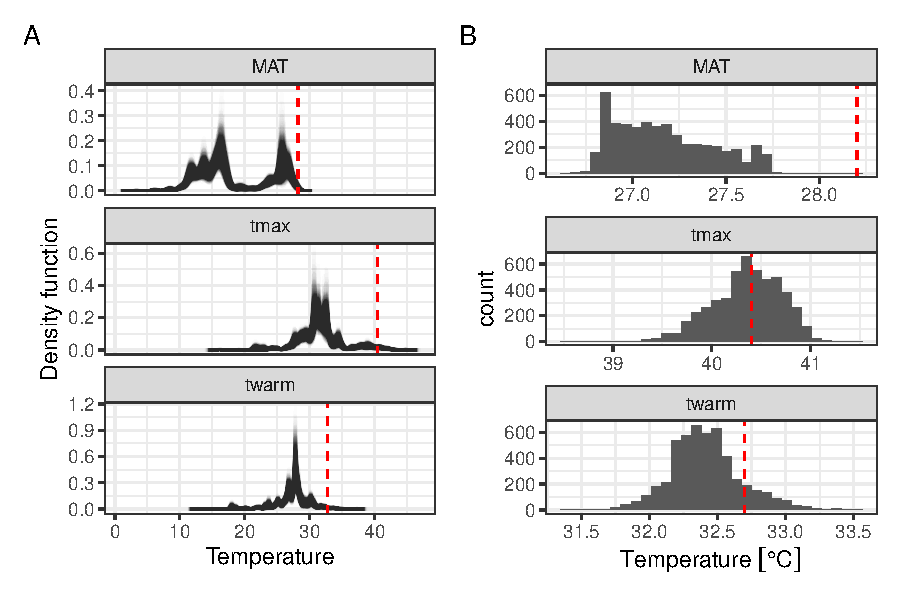
\includegraphics[keepaspectratio]{main_files/figure-pdf/fig-bootstrap-1.pdf}}

}

\caption{\label{fig-bootstrap}A) Bootstrapped kernel density estimates
of rice's thermal extent throughout the Holocene. Bootstrap resampling
accounts for uncertainty in radiocarbon and phase-based dating of
archaeological rice finds. Contemporary temperature thresholds indicated
in red. B) Estimated 97.5\% quantiles from the bootstrapped dataset.
Contemporary quantiles indicated in red.}

\end{figure}%

\newpage{}

\phantomsection\label{cell-fig-recon-timeseries}
\begin{figure}[H]

\centering{

\pandocbounded{\includegraphics[keepaspectratio]{main_files/figure-pdf/fig-recon-timeseries-1.pdf}}

}

\caption{\label{fig-recon-timeseries}Comparison of Holocene temperature
trends over Asia from transient climate models and reconstructions. A)
Holocene trends in mean annual temperature, relative to the 3-5ka mean,
from Osman et al.~2021 (black, one standard deviation uncertainty in
grey), Erb et al.~2022 (blue), and CHELSA-TraCE21k (red). B) Comparison
of annual, seasonal, and monthly temperature trends over Asia from
CHELSA-TraCE21k.}

\end{figure}%

\newpage{}

\phantomsection\label{cell-fig-kde-lgmr}
\begin{figure}[H]

\centering{

\pandocbounded{\includegraphics[keepaspectratio]{main_files/figure-pdf/fig-kde-lgmr-1.pdf}}

}

\caption{\label{fig-kde-lgmr}Kernel density estimates of the thermal
distribution by millennium across two different temperature datasets,
with raw data points indicated in black and contemporary rice thermal
limits in red. A) Temperature data are derived from CHELSA-TraCE21k V1.0
(Karger et al.~2023) (same as Figure 3b in main text). B) Temperature
data derived from the Last Glacial Maximum Reanalysis (LGMR) dataset
(Osman et al.~2022). C) Difference in kernel density estimates of mean
annual temperature (MAT) between the CHELSA-TraCE21k and LGMR datasets.}

\end{figure}%

\newpage{}

\phantomsection\label{cell-fig-country-summaries}
\begin{figure}[H]

\centering{

\pandocbounded{\includegraphics[keepaspectratio]{main_files/figure-pdf/fig-country-summaries-1.pdf}}

}

\caption{\label{fig-country-summaries}Projected increases in land area
surpassing key temperature thresholds in each of the top 15
rice-producing countries in east Asia.}

\end{figure}%

\newpage{}

\phantomsection\label{cell-fig-niche-all-models-bio1}
\begin{figure}[H]

\centering{

\pandocbounded{\includegraphics[keepaspectratio]{main_files/figure-pdf/fig-niche-all-models-bio1-1.pdf}}

}

\caption{\label{fig-niche-all-models-bio1}Predicted changes in mean
annual temperature over currently cultivated rice areas in Asia for
multiple CMIP6 ensemble members.}

\end{figure}%

\newpage{}

\phantomsection\label{cell-fig-niche-all-models-bio10}
\begin{figure}[H]

\centering{

\pandocbounded{\includegraphics[keepaspectratio]{main_files/figure-pdf/fig-niche-all-models-bio10-1.pdf}}

}

\caption{\label{fig-niche-all-models-bio10}Predicted changes in mean
maximum temperature of the warmest quarter over currently cultivated
rice areas in Asia for multiple CMIP6 ensemble members.}

\end{figure}%

\newpage{}

\phantomsection\label{cell-fig-niche-all-models-bio5}
\begin{figure}[H]

\centering{

\pandocbounded{\includegraphics[keepaspectratio]{main_files/figure-pdf/fig-niche-all-models-bio5-1.pdf}}

}

\caption{\label{fig-niche-all-models-bio5}Predicted changes in mean
maximum temperature of the warmest month over currently cultivated rice
areas in Asia for multiple CMIP6 ensemble members.}

\end{figure}%

\newpage{}

\phantomsection\label{cell-fig-displacement}
\begin{figure}[H]

\centering{

\pandocbounded{\includegraphics[keepaspectratio]{main_files/figure-pdf/fig-displacement-1.pdf}}

}

\caption{\label{fig-displacement}Estimated displacement of the optimal
growing location of rice landraces away from the equator, based on
genetic offset analysis across three future temperature scenarios. The
x-axis indicates the difference between the absolute projected latitude
in the future scenario and the absolute latitude today, with positive
values indicating a shift in the optimal growing location of a given
population away from the equator.}

\end{figure}%

\newpage{}

\begin{table}

\caption{\label{tbl-quantiles}Present-day rice extent quantiles (in °C)
across three datasets of varying resolution and spatiotemporal support,
compared to those calculated from archaeological sites in Asia
throughout the Holocene.}

\centering{

\fontsize{12.0pt}{14.4pt}\selectfont
\begin{tabular*}{\linewidth}{@{\extracolsep{\fill}}ccccccccccccc}
\toprule
 & \multicolumn{4}{c}{MAT} & \multicolumn{4}{c}{TMAX} & \multicolumn{4}{c}{TWARM} \\ 
\cmidrule(lr){2-5} \cmidrule(lr){6-9} \cmidrule(lr){10-13}
Quantile & IRRI & Mon. & GBIF & Arch. & IRRI & Mon. & GBIF & Arch. & IRRI & Mon. & GBIF & Arch. \\ 
\midrule\addlinespace[2.5pt]
1.0 [\%] & 3.6 & 4.6 & 3.1 & 8.5 & 23.2 & 22.5 & 17.2 & 22.0 & 19.5 & 18.7 & 13.2 & 18.1 \\ 
2.5 [\%] & 5.6 & 9.1 & 9.1 & 10.3 & 24.9 & 24.8 & 21.2 & 24.2 & 20.5 & 20.8 & 16.8 & 20.0 \\ 
5.0 [\%] & 10.2 & 12.6 & 13.6 & 11.4 & 26.0 & 26.3 & 24.0 & 26.9 & 21.5 & 22.1 & 20.1 & 22.8 \\ 
10.0 [\%] & 13.1 & 15.4 & 16.9 & 11.8 & 27.6 & 27.7 & 26.5 & 28.0 & 23.4 & 23.7 & 22.4 & 24.6 \\ 
90.0 [\%] & 27.2 & 27.3 & 27.8 & 26.5 & 38.4 & 39.1 & 37.8 & 36.5 & 31.5 & 31.9 & 30.7 & 30.3 \\ 
95.0 [\%] & 27.8 & 27.8 & 28.3 & 26.8 & 39.5 & 40.2 & 39.6 & 38.9 & 32.2 & 32.7 & 32.2 & 31.4 \\ 
97.5 [\%] & 28.2 & 28.2 & 28.6 & 27.1 & 40.4 & 40.9 & 40.5 & 40.4 & 32.7 & 33.4 & 33.0 & 32.4 \\ 
99.0 [\%] & 28.6 & 28.6 & 28.9 & 27.7 & 41.0 & 41.7 & 41.4 & 41.0 & 33.1 & 34.6 & 34.4 & 33.4 \\ 
\bottomrule
\end{tabular*}

}

\end{table}%

\newpage{}

\begin{longtable}[]{@{}lrrrr@{}}

\caption{\label{tbl-country-summaries-table1}Projected increases in
percent land area surpassing MAT thresholds in each of the top 15
rice-producing countries in east Asia.}

\tabularnewline

\toprule\noalign{}
Country & Present & SSP1-2.6 & SSP3-7.0 & SSP5-8.5 \\
\midrule\noalign{}
\endhead
\bottomrule\noalign{}
\endlastfoot
Bangladesh & 0 & 0 & 50 & 82 \\
Cambodia & 10 & 75 & 91 & 93 \\
China & 0 & 0 & 0 & 1 \\
India & 4 & 23 & 63 & 75 \\
Indonesia & 0 & 8 & 62 & 69 \\
Japan & 0 & 0 & 0 & 0 \\
Laos & 0 & 6 & 26 & 38 \\
Malaysia & 0 & 11 & 65 & 74 \\
Myanmar & 0 & 15 & 42 & 53 \\
Nepal & 0 & 0 & 7 & 15 \\
Pakistan & 1 & 23 & 52 & 60 \\
Philippines & 0 & 19 & 64 & 72 \\
South Korea & 0 & 0 & 0 & 0 \\
Thailand & 9 & 45 & 79 & 85 \\
Vietnam & 0 & 14 & 38 & 47 \\

\end{longtable}

\newpage{}

\begin{longtable}[]{@{}lrrrr@{}}

\caption{\label{tbl-country-summaries-table2}Projected increases in
percent land area surpassing TWARM thresholds in each of the top 15
rice-producing countries in east Asia.}

\tabularnewline

\toprule\noalign{}
Country & Present & SSP1-2.6 & SSP3-7.0 & SSP5-8.5 \\
\midrule\noalign{}
\endhead
\bottomrule\noalign{}
\endlastfoot
Bangladesh & 0 & 0 & 6 & 42 \\
Cambodia & 0 & 2 & 46 & 63 \\
China & 0 & 0 & 8 & 13 \\
India & 15 & 47 & 66 & 74 \\
Indonesia & 0 & 0 & 0 & 4 \\
Japan & 0 & 0 & 0 & 2 \\
Laos & 0 & 0 & 9 & 19 \\
Malaysia & 0 & 0 & 0 & 6 \\
Myanmar & 0 & 3 & 20 & 33 \\
Nepal & 0 & 0 & 10 & 17 \\
Pakistan & 42 & 57 & 71 & 77 \\
Philippines & 0 & 0 & 3 & 10 \\
South Korea & 0 & 0 & 0 & 0 \\
Thailand & 0 & 5 & 38 & 51 \\
Vietnam & 0 & 0 & 14 & 28 \\

\end{longtable}

\newpage{}

\begin{longtable}[]{@{}lrrrr@{}}

\caption{\label{tbl-country-summaries-table3}Projected increases in
percent land area surpassing TMAX thresholds in each of the top 15
rice-producing countries in east Asia.}

\tabularnewline

\toprule\noalign{}
Country & Present & SSP1-2.6 & SSP3-7.0 & SSP5-8.5 \\
\midrule\noalign{}
\endhead
\bottomrule\noalign{}
\endlastfoot
Bangladesh & 0 & 0 & 0 & 1 \\
Cambodia & 0 & 0 & 13 & 18 \\
China & 0 & 0 & 3 & 6 \\
India & 14 & 39 & 53 & 64 \\
Indonesia & 0 & 0 & 0 & 0 \\
Japan & 0 & 0 & 0 & 0 \\
Laos & 0 & 0 & 2 & 5 \\
Malaysia & 0 & 0 & 0 & 0 \\
Myanmar & 0 & 3 & 10 & 20 \\
Nepal & 0 & 0 & 1 & 8 \\
Pakistan & 36 & 52 & 64 & 71 \\
Philippines & 0 & 0 & 0 & 0 \\
South Korea & 0 & 0 & 0 & 0 \\
Thailand & 0 & 0 & 10 & 18 \\
Vietnam & 0 & 0 & 1 & 5 \\

\end{longtable}




\end{document}
